% =====================================================================
%  consolidated_part_v4.tex
%
%  Updated final report -- adds the threshold-crossing campaign results
%  (Phase B at Re_a/Ha^2 = 6.0 and Phase C at Re_a/Ha^2 = 14.6) and
%  the quantitative empirical 3D transition threshold (Re_a/Ha^2)_c,3D
%  ~ 15 -- a factor of ~4 above the Q2D Sommeria-Moreau prediction.
%
%  Changes from v3:
%   - Abstract updated with the three-point threshold-crossing result.
%   - New Sec V.E "Threshold-crossing campaign" between Q2D and cluster
%     cost subsections.
%   - Discussion VI.A and VI.B substantially strengthened with the
%     factor-of-4 measurement.
%   - Conclusion adds the threshold-crossing as a seventh delivery.
%   - Future work updates the planned saturation campaign.
% =====================================================================

\documentclass[aps,prl,twocolumn,superscriptaddress]{revtex4-2}
\usepackage{graphicx}
\usepackage{amsmath}
\usepackage{xcolor}
\usepackage{url}

\begin{document}

\title{Turbulence Instabilities of a Conducting Fluid in a Corbino Geometry}

\author{Ahmet Eray Kocaman}
\affiliation{Department of Physics, Bilkent University, Bilkent,
06800, Ankara, T\"urkiye}

\date{\today}

\begin{abstract}
We investigate the linear and nonlinear stability of magnetohydrodynamic
(MHD) flow in a Corbino disk of liquid Galinstan (GaInSn) under a
uniform axial magnetic field, at Hartmann number $Ha = 94.88$.  A
custom OpenFOAM solver, \texttt{epotMhdFoam}, extends the
Foundation~13 \texttt{mhdFoam} to the canonical low-magnetic-Reynolds
electric-potential formulation appropriate for an electrode-driven
liquid metal.  The validated $360^{\circ}$ laminar baseline reproduces
six analytical predictions to sub-percent accuracy except for two
physical signatures of the back-EMF self-coupling: a $4\,\%$
deviation of $r\!\cdot\! U_\theta$ from a perfect $1/r$ profile and a
$14\,\%$ shift of $\Phi$ at $r = 4$~cm relative to the pure-Laplace
prediction.  A same-seed five-amplitude perturbation bracket at the
nominal operating point $Re_a/Ha^{2} = 1.19$ establishes nonlinear
stability up to $\alpha = 30\,\%$ RMS amplitude.  A
threshold-crossing campaign at three operating points
$Re_a/Ha^{2} \in \{1.19,\,6.0,\,14.6\}$ yields the dimensionless
decay rate $\sigma\tau_A \in \{-0.30,\,-0.17,\,-0.03\}$, locating
the empirical three-dimensional transition at
$(Re_a/Ha^{2})_{c,\,\rm 3D} \approx 15$.  A Chebyshev-collocation
analysis of the linearised quasi-two-dimensional (Q2D)
Sommeria--Moreau system places the corresponding depth-averaged
threshold at $(Re_a/Ha^{2})_{c,\,\rm Q2D} \approx 3.78$.  The factor
$\sim\!4$ separation between the two thresholds is a direct
quantitative measurement of the three-dimensional damping channels
(pressure-mediated indirect coupling and back-EMF feedback) that the
depth-averaged Q2D reduction discards.  A measured
$\sim\!50\!\times$ cluster-to-laptop cost ratio quantifies the path
to the production direct numerical simulation (DNS).
\\[1ex]
\textbf{Keywords:} Quasi-two-dimensional turbulence, Corbino disk,
magnetohydrodynamics, OpenFOAM, GaInSn.
\end{abstract}

\maketitle


% =====================================================================
\section{Introduction}
% =====================================================================

Turbulence in electrically conducting liquids becomes a dominant
engineering concern at the high power densities relevant to
liquid-metal batteries~\cite{2}, the Pb--Li breeder blankets of the
ITER fusion reactor~\cite{3,4}, and the next-generation
Sn-Li and Galinstan-cooled divertors and first-wall components~\cite{1}.
Within a tokamak blanket, the working liquid serves simultaneously as
the heat-extraction medium and the tritium-breeding agent while
subjected to the reactor's toroidal magnetic field; the resulting MHD
pressure drops, induced quasi-two-dimensional (Q2D) turbulence, and
the formation of Hartmann and Shercliff boundary layers dictate the
thermal-hydraulic efficiency of the entire fusion fuel cycle.  Modeling
these phenomena requires a fully coupled treatment of velocity and
electric potential that goes beyond the laminar
approximation~\cite{5}.

\begin{figure}[h!]
\centering
\includegraphics[width=0.45\textwidth]{iter.png}
\caption{The ITER tokamak under construction at Cadarache.  Operating
near $4$~K and rated for fusion power $\sim\!500$~MW with magnetic
forces equal to two space-launch rockets, ITER motivates the study of
turbulence in conducting fluids under strong axial fields.  Image
credit~\cite{6}.}
\label{fig:iter}
\end{figure}

A direct empirical benchmark for the present numerical work is the
laboratory MHD program of Klein and Poth\'erat at Coventry, which
uses GaInSn-filled Corbino-disk cells under externally imposed
axial magnetic fields and reports a laminar-to-turbulent transition
near $Re_a/Ha^{2}\!\sim\!1$~\cite{pk2014pothklein}.  In both
engineering and laboratory contexts the central question is the
same: how do fluid inertia and Lorentz braking compete to set the
transition between laminar and turbulent regimes, and what is the
structure of the resulting flow?

The present project addresses this question for a controlled
laboratory geometry: a Corbino disk of liquid Galinstan
($\rm Ga_{68.5}In_{21.5}Sn_{10}$) driven by an imposed radial current
between concentric cylindrical electrodes, immersed in a uniform axial
field $\mathbf{B} = B\,\hat{\mathbf{z}}$.  Galinstan is liquid at room
temperature and offers high electrical conductivity
($\sigma \approx 3.46\times 10^{6}\,\rm S\,m^{-1}$), making it the
canonical bench-scale surrogate for the high-temperature alloys
deployed in fusion contexts~\cite{12}.  The work has three stages: a
fully validated laminar baseline (Step~1), a first-look stability
bracket and threshold-crossing campaign on the laptop debug mesh
(Step~2), and a cluster-deployed production DNS (Step~3).  The
cluster handoff package developed here is staged for the production
runs.


% =====================================================================
\section{Physical configuration}
% =====================================================================

The computational domain is the annular disk
$\Omega = \{(r,\theta,z):\, r_{in} \le r \le r_{out},\,
0 \le \theta < 2\pi,\, 0 \le z \le h\}$.  The inner cylinder
$r = r_{in}$ and outer cylinder $r = r_{out}$ are conducting
electrodes; the top and bottom planes $z = 0$ and $z = h$ are
electrical insulators.  The fluid satisfies no-slip on all four walls.
A uniform axial field $\mathbf{B} = B\,\hat{\mathbf{z}}$ is imposed.
Boundary conditions are summarised as
\begin{itemize}
\item Electrodes ($r = r_{in},\, r_{out}$): fixed potential
  $\Phi = V_{in}, V_{out}$; no-slip $\mathbf{u} = 0$.
\item Insulating walls ($z = 0,\, h$): zero normal current
  $\mathbf{n}\!\cdot\!\mathbf{J} = 0$ (forcing radial/azimuthal currents
  in the fluid)~\cite{8}; no-slip $\mathbf{u} = 0$.
\end{itemize}
The aspect ratio $\Gamma = (r_{out} - r_{in})/h$ controls the
relative dominance of the Hartmann (top/bottom) and Shercliff (side)
boundary layers~\cite{2}.  The geometric and physical parameters are
listed in Table~\ref{tab:params}.

\begin{table}[h!]
\centering
\caption{Geometric and physical parameters and the corresponding
dimensionless numbers.  All raw values verified against
\texttt{case\_360\_laminar/constant/physicalProperties} and
\texttt{0/Phi}.  Transport properties of Galinstan from
Morley~\textit{et al.}~\cite{12}.}
\label{tab:params}
\begin{tabular}{|l|l|l|}\hline
symbol & quantity & value \\ \hline
$r_{in}$ & inner electrode radius & $20$~mm \\
$r_{out}$ & outer electrode radius & $100$~mm \\
$h$ & gap height & $10$~mm \\
$B$ & axial magnetic field & $0.5$~T \\
$\rho$ & fluid mass density & $6440$~kg\,m$^{-3}$ \\
$\nu$ & kinematic viscosity & $3.73\!\times\!10^{-7}$~m$^2$\,s$^{-1}$ \\
$\sigma$ & electrical conductivity & $3.46\!\times\!10^{6}$~S\,m$^{-1}$ \\
$\Delta V$ & applied potential (nominal) & $3.703\!\times\!10^{-3}$~V \\
$I_{\rm design}$ & design current & $500$~A \\ \hline
$\Gamma$ & aspect ratio $(r_{out}-r_{in})/h$ & $8$ \\
$Ha$ & Hartmann number & $94.88$ \\
$\delta_H$ & Hartmann-layer thickness $(h/2)/Ha$ & $52.7$~$\mu$m \\
$Rm$ & magnetic Reynolds number & $0.035$ \\
$\tau_A$ & Lorentz/damping time $\rho/(\sigma B^{2})$ & $7.44$~ms \\
$\tau_H$ & Hartmann-layer relaxation time $Ha\,\tau_A$ & $0.71$~s \\
$Re_a$ & annular Reynolds number (nominal) & $1.07\!\times\!10^{4}$ \\
$Re_a/Ha^{2}$ & PK14 control parameter (nominal) & $1.19$ \\ \hline
\end{tabular}
\end{table}

The applied potential $\Delta V = 3.703$~mV is the nominal value
that, by pure-Laplace conduction $\Phi_L(r) = \Delta V \ln(r_{out}/r) /
\ln(r_{out}/r_{in})$, delivers $I_{\rm design} = 500$~A.  The
threshold-crossing campaign of Sec.~\ref{sec:threshold} uses the same
geometry and field but scales $\Delta V$ to drive higher operating
points.  The Hartmann-layer thickness $\delta_H = (h/2)/Ha$ and the
Joule--viscous diffusive scale $\ell_J = \sqrt{\nu\rho/(\sigma B^{2})}$
are algebraically identical: substitution gives
$\ell_J = \sqrt{\mu_{\rm dyn}/(\sigma B^{2})} = \delta_H$.  This
identity is a consequence of the shared diffusive balance --- the
wall-normal scale across which viscous diffusion balances Joule
braking is the same expression as the in-plane scale on which the
same balance holds.


% =====================================================================
\section{Theory}
% =====================================================================

\subsection{Full coupled MHD system in cylindrical coordinates}
\label{sec:full_mhd}

The complete description of the Corbino flow follows
\cite{8} and starts from Ohm's law for a moving conductor,
\begin{equation}
\mathbf{J} = \sigma\bigl(-\nabla\Phi + \mathbf{u}\!\times\!\mathbf{B}\bigr),
\label{eq:ohm_full}
\end{equation}
in which the $\mathbf{u}\!\times\!\mathbf{B}$ term is the induced
electromotive force whose radial component opposes the externally
driven current (the back-EMF).  The Navier--Stokes equation for an
incompressible Newtonian fluid driven by the resulting Lorentz body
force $\mathbf{f}_L = \mathbf{J}\!\times\!\mathbf{B}$ reads
\begin{equation}
\rho\!\left(\partial_t\mathbf{u}+(\mathbf{u}\!\cdot\!\nabla)\mathbf{u}\right)
= -\nabla p + \mu\nabla^{2}\mathbf{u} + \mathbf{f}_{L},
\label{eq:nseom_full}
\end{equation}
in which the four right-hand-side terms are, in order, the local fluid
acceleration, the nonlinear momentum advection that is the source of
turbulent instabilities at high Reynolds number, the pressure gradient
providing the centripetal balance for swirling flow, and the viscous
stress that sets the resolution requirement for the Hartmann and
Shercliff boundary layers.  Any change in $\mathbf{u}$ modifies
$\mathbf{J}$ through (\ref{eq:ohm_full}), which in turn modifies
$\mathbf{f}_L$ in (\ref{eq:nseom_full}); this velocity--potential
feedback loop is what distinguishes liquid-metal MHD from
neutral-fluid hydrodynamics.

Substituting (\ref{eq:ohm_full}) into the solenoidal current
constraint $\nabla\!\cdot\!\mathbf{J} = 0$ (which itself follows from
charge conservation $\nabla\!\cdot\!\mathbf{J} = -\partial_t\rho_{\rm e}$
with $\rho_{\rm e}$ fixed by the imposed potential) and expanding in
cylindrical coordinates yields the charge-conservation
relation~\cite{8}
\begin{equation}
\partial_r u + \frac{u}{r}
\;=\;\bigl(\hat{M} + \alpha_{\omega\tau}\partial_z^{2} + 1/r^{2}\bigr)\Phi,
\label{eq:charge_full}
\end{equation}
in which $\hat{M}$ is the cylindrical Laplace-like operator
\begin{equation}
\hat{M}f \;=\; \frac{1}{r}\partial_r(r\partial_r f) - \frac{f}{r^{2}}
   \;=\; f''+\frac{f'}{r}-\frac{f}{r^{2}},
\label{eq:Mhat}
\end{equation}
and $\alpha_{\omega\tau} = 1 + (\omega_c\tau)^{2}$ encodes the
conductivity anisotropy under the Hall effect.  The left-hand side of
(\ref{eq:charge_full}) is the $\mathbf{u}\!\times\!\mathbf{B}$-induced
current source; the right-hand side is the diffusion of $\Phi$
through the conducting medium.  This relation provides the missing
link between $\mathbf{u}$ and $\mathbf{J}$: the Lorentz force pushes
the fluid, but the resulting motion does not create or destroy charge
--- it only redistributes it according to the laws of
electromagnetism.

A natural characteristic velocity is set by balancing the Lorentz
body force against the viscous stress over the gap height $h$:
\begin{equation}
U_{0} \;=\; \frac{I\,B\,r_{in}}{2\pi\mu\,h},
\label{eq:U0_full}
\end{equation}
where $I$ is the driving current and $\mu$ the dynamic viscosity.
$U_{0}$ provides a dimensional initial guess for iterative solvers.
Non-dimensionalising the steady-state momentum equation with
$f = U_\theta/U_{0}$ converts it into
\begin{equation}
r^{2}f'' + r f' - f + r^{2}\partial_z^{2}f \;=\; -\,r/r_{in}.
\label{eq:f_eq}
\end{equation}
The ratio of magnetic to viscous forces is the Hartmann number
\begin{equation}
Ha \;=\; B\,L\sqrt{\sigma/(\rho\nu)}\;\gg\; 1
   \;\;\Longrightarrow\;\;
\delta_{H} \;\approx\; h/Ha \;\approx\; 0.05~\text{mm};
\label{eq:Ha_full}
\end{equation}
when $Ha \gg 1$ the conducting fluid in the disk core moves
approximately as a rigid body, and viscous shear is confined to the
wall-attached Hartmann layers.  The numerical values of all these
scales for the present geometry are listed in
Table~\ref{tab:params}.

\subsection{Low-$Rm$ approximation}
\label{sec:lowrm}

Two simplifications of the full system of
Sec.~\ref{sec:full_mhd} are appropriate for this geometry and fluid.
First, the magnetic Reynolds number $Rm = \mu_0\sigma U L \approx
3.5\!\times\!10^{-2}$ is well below unity, so the induction equation
can be dropped and $\mathbf{B}$ held fixed at the externally imposed
value~\cite{1,2}.  Second, the Hall coefficient $\alpha_{\omega\tau}$
of (\ref{eq:charge_full}) reduces to unity because the
electron-cyclotron / collision-time product $\omega_c\tau \sim
10^{-4}$ for Galinstan at room temperature in $B = 0.5$~T, so the
conductivity remains isotropic.  The full system of
Sec.~\ref{sec:full_mhd} then reduces to the canonical low-$Rm$
electric-potential formulation used here.

Conservation of mass and momentum for an incompressible Newtonian
fluid driven by a Lorentz body force reads
\begin{align}
\nabla\!\cdot\!\mathbf{u} &= 0, \label{eq:cont}\\
\rho\!\left(\partial_t\mathbf{u} + (\mathbf{u}\!\cdot\!\nabla)\mathbf{u}\right)
&= -\nabla p + \mu\nabla^{2}\mathbf{u} + \mathbf{F}_{L}.
\label{eq:nseom}
\end{align}
Ohm's law in the laboratory frame, after eliminating
the electric field through $\mathbf{E} = -\nabla\Phi$, reads
\begin{equation}
\mathbf{J} = \sigma\bigl(-\nabla\Phi + \mathbf{u}\!\times\!\mathbf{B}\bigr).
\label{eq:ohm_lowrm}
\end{equation}
Charge conservation $\nabla\!\cdot\!\mathbf{J} = 0$ is then a
Poisson-type equation for the electric potential,
\begin{equation}
\nabla\!\cdot\!\bigl(\sigma\nabla\Phi\bigr)
   = \nabla\!\cdot\!\bigl(\sigma\,\mathbf{u}\!\times\!\mathbf{B}\bigr).
\label{eq:phi_poisson}
\end{equation}
The Lorentz body force $\mathbf{F}_L = \mathbf{J}\!\times\!\mathbf{B}$
expanded with~(\ref{eq:ohm_lowrm}) decomposes into three contributions,
\begin{equation}
\mathbf{F}_L = \sigma\bigl[
   -\nabla\Phi\!\times\!\mathbf{B}
   + (\mathbf{u}\!\cdot\!\mathbf{B})\mathbf{B}
   - |\mathbf{B}|^{2}\mathbf{u}\bigr].
\label{eq:lorentz_decomp}
\end{equation}
The first term is the driving force from the imposed potential.  The
second couples to $\mathbf{u}\!\cdot\!\mathbf{B}$, which is small for
an axial field and a predominantly azimuthal velocity.  The third
term is a linear sink with characteristic timescale
$\tau_A = \rho/(\sigma B^{2}) \approx 7.5$~ms; this Hartmann body
damping is much faster than the convective Courant limit on the
present mesh, and an explicit treatment would dominate the cost.  The
standard remedy~\cite{2} is to treat this term implicitly, which in
OpenFOAM is the operator \texttt{fvm::Sp(sigma|B|\^{}2/rho, U)};
the integration timestep is then bounded only by the convective
Courant condition, a $\sim\!25\!\times$ speed-up over the explicit
limit.

\subsection{Linearisation about the laminar base state}
\label{sec:linearise}

Linearising~(\ref{eq:cont})--(\ref{eq:lorentz_decomp}) about a steady
axisymmetric reference state
$\{\mathbf{U}_{0}(r,z),\Phi_{0}(r,z),p_{0}(r,z)\}$ representing the
validated laminar Corbino solution
($\langle U_{\theta,0}\rangle_{z} \propto 1/r$ in the bulk, with the
Hartmann profile~(\ref{eq:hartmann_profile}) below across $z$), and
writing $\mathbf{u} = \mathbf{U}_{0} + \mathbf{u}'$,
$\Phi = \Phi_{0} + \Phi'$, $p = p_{0} + p'$, the system becomes
\begin{align}
\nabla\!\cdot\!\mathbf{u}' &= 0, \label{eq:lin_cont}\\
\nabla\!\cdot\!\bigl(\sigma\nabla\Phi'\bigr)
&= \nabla\!\cdot\!\bigl(\sigma\,\mathbf{u}'\!\times\!\mathbf{B}\bigr),
\label{eq:lin_charge}\\
\rho\frac{\partial\mathbf{u}'}{\partial t}
+ \rho(\mathbf{U}_{0}\!\cdot\!\nabla)\mathbf{u}'
+ \rho(\mathbf{u}'\!\cdot\!\nabla)\mathbf{U}_{0}
&= -\nabla p' + \mu\nabla^{2}\mathbf{u}' + \mathbf{F}_{L}',
\label{eq:lin_mom}
\end{align}
with the linearised Lorentz force
\begin{equation}
\mathbf{F}_{L}' = \sigma\!\left[
   -\nabla\Phi'\!\times\!\mathbf{B}
   + (\mathbf{u}'\!\cdot\!\mathbf{B})\mathbf{B}
   - B^{2}\mathbf{u}'\right].
\label{eq:lin_lorentz}
\end{equation}
With $\mathbf{B} = B\,\hat{\mathbf{z}}$, the last term reads
$-\sigma B^{2}(u'_x, u'_y, 0)$: only the in-plane components are damped
directly at rate $\tau_A^{-1}$.  The axial component $u'_z$ feels the
body force only indirectly --- through pressure-mediated coupling to
$\mathbf{u}'_\perp$ via continuity~(\ref{eq:lin_cont}), and through the
back-EMF feedback via~(\ref{eq:lin_charge})~\cite{1,2}.  This
symmetry-driven structure is what bounds the dimensionless decay rate
$|\sigma\tau_A|$ below the direct body-force value of unity, and is
what is observed empirically in Sec.~\ref{sec:bracket} and in the
threshold-crossing campaign of Sec.~\ref{sec:threshold}.

\subsection{Quasi-two-dimensional reduction}
\label{sec:q2d}

For $Ha\!\gg\!1$ the Hartmann layers are exponentially thin
($\delta_H/h \sim 1/Ha \approx 10^{-2}$ here) and the bulk
perturbation is approximately columnar in $z$.  Depth-averaging
(\ref{eq:lin_cont})--(\ref{eq:lin_mom}) over $z\in[0,h]$ and applying
the asymptotic Hartmann-layer wall-shear closure
$\tau_w = \rho U_\infty\sqrt{\mu\sigma B^{2}}/\rho$ produces the
Sommeria--Moreau Q2D system~\cite{9}:
\begin{align}
\nabla_{2}\!\cdot\!\langle\mathbf{u}'\rangle_{z} &= 0, \\
\rho\partial_t\langle\mathbf{u}'\rangle_{z}
&+ \rho(\langle\mathbf{U}_{0}\rangle_{z}\!\cdot\!\nabla_{2})
   \langle\mathbf{u}'\rangle_{z}
   \nonumber \\
&+ \rho(\langle\mathbf{u}'\rangle_{z}\!\cdot\!\nabla_{2})
   \langle\mathbf{U}_{0}\rangle_{z}
   \nonumber\\
&= -\nabla_{2}\langle p'\rangle_{z}
   + \mu\nabla_{2}^{2}\langle\mathbf{u}'\rangle_{z}
   - \frac{\rho}{\tau_{H}}\langle\mathbf{u}'\rangle_{z},
   \label{eq:sm_mom}
\end{align}
with $\nabla_{2} = (\partial_r,\, r^{-1}\partial_\theta)$ the in-plane
gradient and $\tau_{H} = Ha\,\tau_A$ the Hartmann friction time.  The
Hartmann friction term $-(\rho/\tau_H)\langle\mathbf{u}'\rangle_{z}$
replaces the volumetric body damping of (\ref{eq:lin_lorentz}) and
captures the depth-integrated effect of the wall-layer drag at
leading order in $1/Ha$~\cite{2}.  Note that this depth-averaging
discards both indirect damping channels of
Sec.~\ref{sec:linearise} --- the pressure-mediated $u'_z$ coupling
and the volumetric back-EMF feedback --- and therefore systematically
underestimates the true 3D damping rate.  This systematic bias is
quantified empirically in Sec.~\ref{sec:threshold}.

The axisymmetry of the base state $\langle U_{\theta,0}\rangle_{z}(r)$
makes the linearised operator separable in $\theta$.  Substituting the
Fourier ansatz
$\langle u'_{i}(r,\theta,t)\rangle_{z}
   = \hat{u}_{i}(r)\,\exp(\sigma t + i m\theta)$
with $m\!\in\!\mathbb{Z}_{\ge 1}$ into~(\ref{eq:sm_mom}) and using
continuity to eliminate $\hat{u}_r$ reduces the system to a
one-dimensional generalised eigenvalue problem,
\begin{equation}
\sigma\,\hat\psi_{m}(r) = \mathcal{L}_{m}\bigl[
   \langle U_{\theta,0}\rangle_{z};\,Ha,Re_{a}\bigr]\,\hat\psi_{m}(r),
\label{eq:eigenvalue}
\end{equation}
in the radial streamfunction $\hat\psi_{m}$.  The operator
$\mathcal{L}_{m}$ combines the inertial coupling to the base-flow
shear, viscous diffusion in $r$, the Hartmann friction $-1/\tau_H$,
and the back-EMF feedback through the depth-averaged $\Phi'$
equation~\cite{8}.  Boundary conditions are
$\hat\psi_{m}(r_{in}) = \hat\psi_{m}(r_{out}) = 0$ (no-slip at the
electrode walls); these are extended to clamped streamfunction
$\hat\psi = \hat\psi' = 0$ to enforce zero radial flux at both
electrodes.

\subsection{Two analytical observations}
\label{sec:q2d_obs}

Two analytical features of the linearised Q2D Corbino problem deserve
note before turning to the numerical solution.

First, the laminar base state $\langle U_{\theta,0}\rangle_{z}(r)
= K/r$ is irrotational in the bulk:
\begin{equation}
\Omega_{0}(r) = \frac{1}{r}\frac{d(r\,U_{\theta,0})}{dr}
   = \frac{1}{r}\frac{dK}{dr} = 0,
\label{eq:omega0_zero}
\end{equation}
so the shear-coupling term
$(\mathbf{u}'\!\cdot\!\nabla_{2})\Omega_{0}$ in the linearised
vorticity equation vanishes identically.

Second, the radial profile of the convective Doppler shift
$im\,U_{\theta,0}/r = imK/r^{2}$ varies across the gap because the
base flow is differentially rotating.  The advection operator
$im(K/r^{2})$ does not commute with the modal Laplacian $L_{m}$; the
linearised operator is therefore non-normal in the sense of
Trefethen--Embree, and its eigenvalues are not given by the simple
Hermitian/anti-Hermitian decomposition.  In particular,
$\Re(\sigma)$ is not pinned to the Hartmann-friction value $-1/\tau_H$
and can be shifted toward zero by the non-normality.  The
quantitative consequences are computed in Sec.~\ref{sec:results_q2d}.


% =====================================================================
\section{Methods}
% =====================================================================

\subsection{Custom solver: \texttt{epotMhdFoam}}

OpenFOAM Foundation's stock \texttt{mhdFoam} solves the induction
equation for $\mathbf{B}$ and uses the Maxwell stress as the body
force.  For a uniform axial $\mathbf{B}$, however,
$\nabla\!\times\!\mathbf{B}\equiv 0$ in the bulk, the Lorentz force is
identically zero, and the fluid does not move.  An eight-hour
\texttt{mhdFoam} run on the present case produced
$|\mathbf{u}|\sim 10^{-13}$~m/s, confirming this failure mode
empirically.  The Corbino fluid is driven by an \emph{imposed
potential} through the electrodes, not by induction; the canonical
low-$Rm$ electric-potential formulation~\cite{1,2} of
Sec.~\ref{sec:lowrm} provides the missing physics.

The custom solver \texttt{epotMhdFoam} extends \texttt{mhdFoam} by:
\textit{(i)} removing the induction equation and its
magnetic-pressure correction loop; \textit{(ii)} adding the
$\Phi$-Poisson equation~(\ref{eq:phi_poisson}); and
\textit{(iii)} replacing the Maxwell-stress body force with the
explicit Lorentz decomposition~(\ref{eq:lorentz_decomp}), the
Hartmann-damping term treated implicitly via \texttt{fvm::Sp}.  The
implementation is approximately 200 lines of OpenFOAM code organised
into \texttt{epotMhdFoam.C} (main loop), \texttt{createFields.H}
(field registration with correct SI dimensions), \texttt{PhiEqn.H}
(the Poisson solve), and \texttt{createControl.H} (PISO control).
The build is by \texttt{wmake} against the Foundation~13 toolkit.

\subsection{Numerical settings}

\subsubsection*{Adaptive time-stepping}
The PISO loop has no built-in \texttt{setDeltaT.H}; an inline
Courant-based controller is written into the main loop, with maximum
Courant number $\mathrm{Co}_{\max}$ set in \texttt{controlDict} and
\texttt{runTimeModifiable yes} permitting live retuning.  At
$\mathrm{Co}_{\max} = 0.5$ on the laptop debug mesh
($\Delta z_{\min} = 50~\mu$m, $|\mathbf{u}|\sim 0.1$~m/s) this yields
$\Delta t \approx 2\!\times\!10^{-4}$~s.  A hard cap
$\Delta t_{\max} = 5\!\times\!10^{-4}$~s prevents pathological
overshoots in transient regions where the Courant estimator
under-reports.

\subsubsection*{Linear-solver tuning: GAMG-$\Phi$}
A non-default linear-solver tuning is required for the $\Phi$-Poisson
equation.  The OpenFOAM default for symmetric positive-definite
Poisson operators is \texttt{PCG} with \texttt{DIC} preconditioning.
On the closed Corbino domain --- bounded by mostly-insulating walls,
with Dirichlet conditions only on the inner and outer electrodes
($\sim 5\,\%$ of the surface area) --- the default produced 320--400
PCG iterations per timestep to drive the residual from $\mathcal{O}(1)$
(cold start) to $10^{-8}$.  Switching to \texttt{GAMG} with
\texttt{DICGaussSeidel} smoothing reduces the iteration count to
2--5 per timestep at the same tolerance, a $5$--$10\!\times\!$
wall-clock speed-up on the debug mesh.

The mechanism is geometric: the closed-domain $\Phi$ field carries
slow-decaying low-frequency modes that DIC-preconditioned CG resolves
only by iterating across the whole domain; GAMG's geometric coarsening
collapses them in a few V-cycles.  This tuning does not transfer to
the $\mathbf{U}$ momentum solver, which remains on
\texttt{PBiCGStab/DILU} because its operator is advection-dominated.

\subsubsection*{Discretisation schemes}
Time integration uses second-order \texttt{backward}, A-stable and
canonical for adaptive-$\Delta t$ PISO at $\mathrm{Co}_{\max}\le 0.5$.
Spatial discretisation uses \texttt{Gauss linear corrected} Laplacian
and gradient schemes (second-order on hexahedral meshes, with
non-orthogonal correction at the wall-grading transition).  Momentum
advection uses \texttt{Gauss limitedLinearV 1} for the production
case; \texttt{Gauss linear} suffices for the laminar baseline.  PISO
parameters are $n_{\rm corr} = 2$, $n_{\rm nonOrtho} = 1$.

\subsection{Mesh strategy}

\subsubsection*{Topology}
The mesh is a four-block hexahedral O-grid covering the full
$360^{\circ}$ annulus.  Each block spans one quadrant
$\theta\in[k\!\cdot\!90^{\circ},(k+1)\!\cdot\!90^{\circ}]$,
$k\in\{0,1,2,3\}$, sharing inner and outer cylindrical arc edges with
adjacent blocks.  Vertices, edges, and patches are inherited from the
laminar baseline mesh; only cell counts and the $z$-grading vary
across the hierarchy in Table~\ref{tab:meshes}.

\begin{table}[h!]
\centering
\caption{Mesh hierarchy used in this work.}
\label{tab:meshes}
\begin{tabular}{|l|c|c|c|c|}\hline
mesh & $N_r$ & $N_\theta$ & $N_z$ & total cells \\ \hline
debug (under-resolved) & 200 & 96 & 30 & $2.30\!\times\!10^{6}$ \\
debug Hartmann-resolved & 200 & 64 & 70 & $3.58\!\times\!10^{6}$ \\
production (medium) & 600 & 384 & 70 & $6.45\!\times\!10^{7}$ \\ \hline
\end{tabular}
\end{table}

\begin{figure}[h!]
\centering
\includegraphics[width=0.45\textwidth]{disc1.png}
\caption{The full-$360^{\circ}$ mesh used for the laminar baseline,
visualised in ParaView.  Four hexahedral O-grid blocks cover the
annulus; only one quadrant is highlighted to expose the topology.}
\label{fig:mesh}
\end{figure}

\subsubsection*{$z$-grading and the Hartmann criterion}
The DNS-grade $z$-grading uses three segments: an 11-cell geometric
stack at each Hartmann wall with first-cell height
$\Delta z_{\min} = 7~\mu$m and expansion ratio $q = 1.2$, plus a
48-cell uniform bulk segment.  Cumulative wall-cell heights are
$7.0,\, 15.4,\, 25.5,\, 37.6,\, 52.1,\, 69.5\,\mu$m: the fifth cell
ends just below $\delta_H = 52.7~\mu$m, satisfying the
``$\ge 5$ cells in $\delta_H$'' criterion that has become standard for
wall-resolved Hartmann channel DNS~\cite{2}.  The wall-cluster span is
$225~\mu$m, the bulk-segment span is $9.55$~mm, and total
$N_z = 11 + 48 + 11 = 70$.

\subsubsection*{Under-resolved laptop variant}
For the Step-2 first-look stability bracket and the threshold-crossing
campaign of Sec.~\ref{sec:threshold}, an under-resolved variant with
$\Delta z_{\min} = 50~\mu$m, $q = 1.3$, and $N_z = 30$ was used.
This mesh fits in laptop RAM, and the convective Courant limit allows
$\Delta t \approx 5\!\times\!10^{-4}$~s, ten times larger than the
Hartmann-resolved limit.  The cost of the resolution shortfall is
quantified in Sec.~\ref{sec:cluster}.

\subsection{Verification criteria}
\label{sec:verif}

Two laminar-regime invariants serve as success criteria for the
Step-1 baseline and as monitors during the perturbation runs.

\textit{(a) Symmetry of the Lorentz force.}  In the laminar Corbino
state with $\mathbf{u}\!\approx\!u_\theta\hat{\boldsymbol\theta}$ and
$\mathbf{B} = B\hat{\mathbf{z}}$, the current density $\mathbf{J}$ is
predominantly radial and the body force
$\mathbf{J}\!\times\!\mathbf{B}$ is therefore predominantly azimuthal.
Any induced azimuthal current
$J_\theta = \sigma(\mathbf{u}\!\times\!\mathbf{B})_\theta$ would
generate a spurious radial force.  The dimensionless symmetry
verification ratio
\begin{equation}
\epsilon_{\rm sym} \;=\; |f_r|/|f_\theta|
\label{eq:eps_sym}
\end{equation}
must satisfy $\epsilon_{\rm sym} < 10^{-3}$ for the laminar
interpretation to hold~\cite{2}.  Once turbulence develops,
$\mathbf{J}$ acquires azimuthal and axial components, $\mathbf{f}_L$
develops radial and axial components, and $\epsilon_{\rm sym}$ rises
sharply --- so the same metric serves as a sensitive monitor for the
onset of three-dimensional motion.

\textit{(b) Global torque conservation.}  The total Lorentz torque
applied to the fluid volume satisfies analytically
\begin{equation}
\tau_{\rm ana}
   \;=\; \int_{0}^{h}\!\!\int_{0}^{2\pi}\!\!\int_{r_{in}}^{r_{out}}\!
        (r\,f_\theta)\,r\,dr\,d\theta\,dz
   \;=\; \tfrac{1}{2}\,I\,B\,(r_{out}^{2} - r_{in}^{2}),
\label{eq:torque_ana}
\end{equation}
and is computed numerically in Cartesian components as~\cite{2}
\begin{equation}
\tau_{\rm num} \;=\; \iiint_\Omega (x\,f_y - y\,f_x)\,dx\,dy\,dz.
\label{eq:torque_num}
\end{equation}
The model is verified when
$E_\tau = |\tau_{\rm num} - \tau_{\rm ana}|/\tau_{\rm ana} < 0.01$,
confirming that the total power injected into the fluid is
physically correct before the introduction of turbulent dissipation.
The Step-1 measurement (Sec.~\ref{sec:results_step1}) returns
$E_\tau = 0.0054$, well inside the budget.

\subsection{Initial-condition injection}
\label{sec:ic_injection}

The Step-2 stability test injects a divergence-free vortical
perturbation $\mathbf{u}'$ onto the converged Step-1 laminar field at
$t = t_0$.  The construction is in three stages.

\subsubsection*{Spectral construction}
A random Gaussian vector potential $\boldsymbol{\psi}(\mathbf{x})$ is
drawn on a Cartesian grid covering the annulus (with padding factor
$1.5$).  The grid is sized so that the integral scale $L_{int} =
5$~mm is resolved by approximately six points.  $\boldsymbol{\psi}$
is filtered through the Pope--Passot--Pouquet spectrum
\begin{equation}
E(k) \propto (k/k_p)^{4}\,\exp\!\bigl(-2(k/k_p)^{2}\bigr),
\label{eq:spec}
\end{equation}
peaked at $k_p = 2\pi/L_{int}$.  This form has the convenient
analytical property that energy is concentrated at the integral
scale and decays smoothly at both ends, avoiding the truncation
ringing of a top-hat spectrum.  The perturbation velocity is
constructed as
\begin{equation}
\mathbf{u}'(\mathbf{x}) = \nabla\!\times\!\boldsymbol{\psi}(\mathbf{x}),
\label{eq:curl}
\end{equation}
which satisfies $\nabla\!\cdot\!\mathbf{u}' \equiv 0$ exactly.  The
field is interpolated trilinearly onto the OpenFOAM cell centres.

\subsubsection*{Wall taper}
A multiplicative envelope is applied to make $\mathbf{u}'$ vanish at
all four no-slip walls,
\begin{equation}
T(r,z) = \sin\!\Bigl(\pi\frac{r-r_{in}}{r_{out}-r_{in}}\Bigr)\,
        \sin\!\Bigl(\pi\frac{z}{h}\Bigr).
\label{eq:taper}
\end{equation}
This taper breaks the divergence-free property to leading order in
$L_{taper}/L_{int}\!\sim\!1\,\mathrm{mm}/5\,\mathrm{mm}$.  The
residual $\nabla\!\cdot\!\mathbf{u}'$ is cleaned up by the first PISO
pressure-correction sweep at restart, observed in the solver log as
a single transient with elevated $p$ initial residual on the first
timestep, returning to the converged-laminar level within 3--5
timesteps.

\subsubsection*{Same-seed amplitude bracket protocol}
After the wall taper, the field is rescaled by a single global
scalar to hit the prescribed RMS amplitude
\begin{equation}
\frac{\langle|\mathbf{u}'|^{2}\rangle^{1/2}}
     {\langle|\mathbf{u}_{lam}|^{2}\rangle^{1/2}} = \alpha,
\label{eq:rms}
\end{equation}
with $\alpha \in \{0.02, 0.05, 0.10, 0.15, 0.30\}$.  All five
amplitudes share the random seed $1729$, so the perturbation field at
each amplitude is exactly a global rescaling of the same underlying
realisation.  This protocol eliminates the seed-mixture confound that
an independent-realisation bracket would introduce.  For each
amplitude, the laminar field at $t_0 = 0.5$~s is reloaded from the
backup \texttt{0.5/U.lam}, perturbed, decomposed across eight ranks,
and integrated for 50~ms.  The same protocol is reused for the
threshold-crossing campaign of Sec.~\ref{sec:threshold} at the
higher operating points.  The implementation is
\texttt{corbino\_turbulance\_debug/scripts/perturb\_ic.py},
$\sim\!280$ lines of NumPy, deterministic for a fixed seed.


% =====================================================================
\section{Results}
\label{sec:results}
% =====================================================================

\subsection{Step-1: validated laminar baseline at $360^{\circ}$}
\label{sec:results_step1}

The Step-1 laminar baseline was integrated to $t = 1.5$~s on a
$307\,200$-cell $360^{\circ}$ mesh, $2531$ timesteps, $79$~min wall
clock on a single i5-1240P core.  Eight observables were extracted
from the final state and a final-window time-mean; the comparison to
analytical predictions is summarised in
Table~\ref{tab:step1_validation}.

\begin{table*}[h!]
\centering
\caption{Step-1 laminar validation against analytical predictions.
All numbers at $t = 1.5$~s, mid-plane unless stated; the relative
error column reports
$|\text{simulated}-\text{predicted}|/\text{predicted}$ where
applicable.}
\label{tab:step1_validation}
\begin{tabular}{|l|l|l|l|}\hline
observable & analytical prediction & simulated & relative error \\ \hline
$U_\theta(r=6$~cm$)$, mid-plane &
$0.099$~m/s ($I_{\rm eff}\!\approx\!632$~A) & $-0.097$~m/s & $2\,\%$ \\
$r\!\cdot\!U_\infty$ peak-to-peak spread & $0$ (perfect $1/r$) & $4\,\%$ &
physical (back-EMF) \\
Hartmann profile RMS error (bulk) & $0$ &
$0.29$--$0.30\,\%$ of $U_\infty$ & discretisation \\
axisymmetry residual
$\max_\theta|U_\theta-\langle U_\theta\rangle_\theta|/U_\infty$ &
$0$ & $\sim\!10^{-4}$ & numerical \\
torque closure $T_{\rm EM}+T_{\rm visc}$ & $0$ & $0.54\,\%$ & converged \\
$\Phi$ at $r = 4$~cm & $2.21$~mV (Laplace) & $2.518$~mV & $14\,\%$ \\
$|U_z|/|U_\theta|$ noise floor (laminar) & $0$ (symmetry) & $\sim 10^{-7}$ &
numerical \\
$|U_r|/|U_\theta|$ noise floor (laminar) & $0$ (symmetry) & $\sim 10^{-4}$ &
corner B\"odewadt \\ \hline
\end{tabular}
\end{table*}

\subsubsection*{Bulk magnitude and the back-EMF excess current}
The simulated $U_\theta(r=6\,\rm cm) = -0.097$~m/s, inverted through
$U_\theta = I/(2\pi r h \sigma B)$, returns
$I_{\rm eff} \approx 632$~A: a $26\,\%$ excess above the
$I_{\rm design} = 500$~A delivered by pure-Laplace conduction.  This
is not a numerical error.  The Lorentz body
force~(\ref{eq:lorentz_decomp}) drives a non-trivial radial deviation
of $U_\theta$ from a perfect $K/r$ profile near the electrodes; the
resulting $\mathbf{u}\!\times\!\mathbf{B}$ source on the right-hand
side of~(\ref{eq:phi_poisson}) deforms $\Phi(r)$ away from the
Laplace shape; the radial current that the modified $\Phi$ profile
delivers is larger than the Laplace estimate would predict.  The same
physics is documented quantitatively as the $14\,\%$ shift of $\Phi$
at $r = 4$~cm and the $4\,\%$ deviation of $r\!\cdot\!U_\theta$ from
$1/r$ in Table~\ref{tab:step1_validation}: all three rows are
signatures of the same self-consistent low-$Rm$ coupling that
distinguishes the moving-fluid solution from the pure-electrostatic
one.

\subsubsection*{Two-timescale spin-up}
The time evolution of $U_\theta$ at the three radial probes exhibits
the predicted two-timescale structure: a fast Alfv\'en/Lorentz phase
reaching $\sim\!80\,\%$ of $U_\infty$ within $\sim\!10\,\tau_A$,
followed by a slow Hartmann-layer relaxation phase with
e-folding time $\sim\tau_H = 0.71$~s.  A two-exponential fit
\begin{equation}
U_\theta(t) = U_\infty - A_A\exp(-t/\tau_A) - A_H\exp(-t/\tau_H)
\label{eq:two_exp}
\end{equation}
with $\tau_A$ locked at the analytical value and four free parameters
returns $\tau_H$ within $\pm 15\,\%$ of $0.71$~s at all three radii.

\subsubsection*{Hartmann profile recovery}
Line probes of $U_\theta(z)$ at $r = 4,\,6,\,8$~cm match the
analytical Hartmann channel profile~\cite{1}
\begin{equation}
U_\theta(z) = U_\infty\!\left[1 - \frac{\cosh\!\bigl((z-h/2)/\delta_H\bigr)}
                                          {\cosh(Ha)}\right],
\label{eq:hartmann_profile}
\end{equation}
with $U_\infty$ anchored at the centreline value (no fit parameter
--- at $z = h/2$ the cosh ratio is $1/\cosh(94.88)\sim 10^{-41}$, so
the centreline numerical value \emph{is} $U_\infty$ to machine
precision).  The bulk RMS error
($z\in[5\delta_H,\,h-5\delta_H]$) is $0.29$--$0.30\,\%$ of $U_\infty$
at every radius.

\subsubsection*{Global torque closure}
Direct integration of the volumetric Lorentz torque
\begin{equation}
T_{\rm EM} = \int_V r\,(\mathbf{J}\!\times\!\mathbf{B})_\theta\,dV,
\label{eq:tem}
\end{equation}
and the wall-shear torque on the two insulating Hartmann plates
\begin{equation}
T_{\rm visc} = \int_{\partial V} r\,\tau_{w\theta}\,dA,
\label{eq:tvisc}
\end{equation}
gives $T_{\rm EM} = -1.2871\!\times\!10^{-2}$~N\,m and
$T_{\rm visc} = +1.2801\!\times\!10^{-2}$~N\,m, a closure
$|T_{\rm EM}+T_{\rm visc}|/\max(|T_{\rm EM}|,|T_{\rm visc}|) =
0.54\,\%$.  The radial split of $T_{\rm EM}$ at the midpoint
$R_{\rm mid} = 6$~cm is $35\,\%$ inner / $65\,\%$ outer, matching the
$1\!:\!2$ annular-volume ratio at that radius and confirming uniform
torque density per unit volume.

\subsubsection*{The $\Phi$ back-EMF: signature of the low-$Rm$ coupling}
At $r = 4$~cm the simulation reads $\Phi = 2.518$~mV against a
pure-Laplace prediction $\Phi_L =
\Delta V\,\ln(r_{out}/r)/\ln(r_{out}/r_{in}) = 2.21$~mV: a $14\,\%$
excess.  This excess is the $\mathbf{u}\!\times\!\mathbf{B}$
contribution to the right-hand side of~(\ref{eq:phi_poisson}).  For
perfect $U_\theta\!\propto\!1/r$ the divergence vanishes; the small
radial deviations of $U_\theta$ from $1/r$ near the electrodes
(themselves caused by the Shercliff side layers~\cite{2} and the
back-EMF self-consistency) produce the finite offset.  The
phenomenon was noted analytically by Keser~\cite{8} as the
radial-deviation correction; to my knowledge no published
Corbino-MHD study has isolated it numerically as a $14\,\%$ effect
at the geometry-relevant Hartmann numbers.

% --------------------------------------------------------------------
\subsection{Step-2: amplitude bracket on the debug mesh}
\label{sec:bracket}

The five-amplitude same-seed bracket was integrated for $50$~ms
($\sim\!6.76\,\tau_A$) starting from the converged laminar IC at
$t = 0.5$~s on the $2.30\!\times\!10^{6}$-cell debug mesh, at the
nominal operating point $Re_a/Ha^{2} = 1.19$.  The
across-probe RMS axial velocity $\langle U_z^{2}\rangle^{1/2}$ is the
cleanest perturbation diagnostic: $U_z\equiv 0$ identically in the
laminar Hartmann state by symmetry, so any non-zero $U_z$ is a pure
perturbation signal with no need to subtract a slowly-drifting
laminar baseline.  A log-linear fit of
$\log\langle U_z^{2}\rangle^{1/2}(t)$ extracts the instantaneous
decay (or growth) rate $\sigma$, and the dimensionless combination
$\sigma\tau_A$ measures this rate against the natural timescale of
the system.

\begin{table*}[h!]
\centering
\caption{Same-seed five-amplitude bracket on the debug mesh, seed
$1729$.  $\langle U_z^{2}\rangle^{1/2}$ in $\rm mm\,s^{-1}$;
$\sigma\tau_A$ dimensionless; e-folding time in milliseconds.}
\label{tab:bracket}
\begin{tabular}{|c|c|c|c|c|c|c|}\hline
amplitude $\alpha$ & init.\ RMS $U_z$ & final RMS $U_z$ &
ratio fin/init & $\sigma\tau_A$ & $R^{2}$ & e-fold (ms) \\ \hline
$0.02$ & $3.19$  & $0.37$ & $0.116$ & $-0.298$ & $0.81$ & $24.9$ \\
$0.05$ & $7.97$  & $0.87$ & $0.109$ & $-0.310$ & $0.84$ & $23.9$ \\
$0.10$ & $15.94$ & $1.56$ & $0.098$ & $-0.332$ & $0.87$ & $22.3$ \\
$0.15$ & $23.91$ & $2.06$ & $0.086$ & $-0.353$ & $0.91$ & $21.0$ \\
$0.30$ & $47.81$ & $2.89$ & $0.060$ & $-0.404$ & $0.95$ & $18.3$ \\ \hline
\end{tabular}
\end{table*}

The bracket data are summarised in the four-panel diagnostic of
Fig.~\ref{fig:bracket_overview} and the amplitude scan of
Fig.~\ref{fig:sigma_amp}.

\begin{figure*}[h!]
\centering
\includegraphics[width=0.85\textwidth]{bracket_overview.png}
\caption{Stability of the laminar Corbino base state at
$Re_a/Ha^{2}\!\approx\!1.19$ from the same-seed five-amplitude bracket.
\textbf{(a)} Time evolution of the across-probe RMS axial velocity
$\langle U_z^{2}\rangle^{1/2}$.  Colour denotes amplitude
$\alpha = 2,5,10,15,30\,\%$.  All amplitudes decay; the ordering is
preserved at every time.  \textbf{(b)} Dimensionless decay rate
$\sigma\tau_A$ as a function of $\alpha$; colour denotes $R^{2}$ of
the log-linear fit.  Dotted line marks $\sigma\tau_A = -1$, the
direct-coupling Hartmann body-force rate that $U_\perp$ would feel.
\textbf{(c)} Back-EMF response amplitude
$\langle\Phi'^{2}\rangle^{1/2}/(U'_z B L_{int})$ vs $\alpha$
(reproduced from the three-amplitude back-EMF run; see
Sec.~\ref{sec:backemf}).  \textbf{(d)} Final/initial ratio
$U_z^{\rm fin}/U_z^{\rm ini}$ at $t-t_0 = 50$~ms; growth threshold
(red dashed) is unity, all amplitudes well below.}
\label{fig:bracket_overview}
\end{figure*}

\begin{figure}[h!]
\centering
\includegraphics[width=0.45\textwidth]{sigma_vs_amplitude.png}
\caption{$\sigma\tau_A$ vs perturbation amplitude.  The data are
monotone in $\alpha$; the dotted line at $\sigma\tau_A = -1$ marks
the direct Hartmann body-force rate, well below the measured
asymptote.  Linear extrapolation reaches that rate only near
$\alpha\!\approx\!200\,\%$, an unphysical amplitude.}
\label{fig:sigma_amp}
\end{figure}

Three monotone trends emerge in lockstep across the
$15\!\times\!$ amplitude span $\alpha\!=\!0.02\!\to\!0.30$:

\textit{Trend (a) --- $\sigma\tau_A$ becomes more negative.}
$\sigma\tau_A$ moves from $-0.298$ to $-0.404$, a $35\,\%$
acceleration of the decay rate.  This is the signature of nonlinear
self-damping: weak mode--mode coupling at finite amplitude mixes the
slow-decaying $U_z$ bottleneck mode into faster, body-force-coupled
$U_\perp$ modes.

\textit{Trend (b) --- $R^{2}$ rises with amplitude.}  The log-linear
fit quality climbs $0.81\!\to\!0.95$ across the same span.  At small
amplitude the decay is a multi-mode sum (poor exponential fit because
modes with different rates contribute additively); at larger amplitude
nonlinear coupling redistributes energy among modes, homogenising the
mixture into a single dominant survivor with cleanly exponential
decay.

\textit{Trend (c) --- final/initial ratio decreases.}  The fraction
of perturbation energy surviving 50~ms decreases
$0.116\!\to\!0.060$, a direct kinematic consequence of trend (a).

\subsubsection*{Stability verdict at the nominal operating point}
\textit{No amplitude in $[2\,\%, 30\,\%]$ shows growth, saturation,
or any non-monotone behaviour.}  The most aggressive perturbation
($\alpha = 0.30$, peak local $U_z$ exceeding $55\,\%$ of laminar
$U_\theta$ at probe locations) collapses to $6\,\%$ of its starting
amplitude in $50$~ms.  The laminar Corbino base state at
$Re_a/Ha^{2}\!\approx\!1.19$ is therefore \textit{nonlinearly stable
to bulk vortical perturbations up to at least $30\,\%$ RMS amplitude},
on the under-resolved debug mesh.  Whether this stability persists
at higher driving is the question addressed in
Sec.~\ref{sec:threshold}.

% --------------------------------------------------------------------
\subsection{Back-EMF linearity}
\label{sec:backemf}

A separate three-amplitude bracket
($\alpha = 0.02,\,0.05,\,0.10$; seeds $1730,\,1729,\,1731$) tracked
the induced potential $\Phi'(t) = \Phi(t) - \Phi_{\rm lam}$ at the
five probes.  An eddy-scale estimate of the back-EMF magnitude is
\begin{equation}
\Phi_{\rm scale} = |\mathbf{u}'_z|_{\rm RMS}\,B\,L_{int};
\label{eq:phi_scale}
\end{equation}
the realised RMS $\Phi'$ divided by this scale gives a dimensionless
\emph{back-EMF efficiency} that approaches unity for a local
single-eddy estimate and falls below unity in a closed
Poisson-smoothed domain.  Results are in Table~\ref{tab:bemf} and
Fig.~\ref{fig:bemf}.

\begin{table}[h!]
\centering
\caption{Back-EMF response across three perturbation amplitudes.
Peak $\Phi'$ in $\mu$V; all ratios dimensionless.}
\label{tab:bemf}
\begin{tabular}{|c|c|c|c|}\hline
$\alpha$ & peak $\Phi'$ & peak $\Phi'/\Phi_{\rm lam}$ &
$\langle\Phi'\rangle_{\rm RMS}/\Phi_{\rm scale}$ \\ \hline
$0.02$ & $1.64$ & $0.120\,\%$ & $0.225$ \\
$0.05$ & $2.23$ & $0.163\,\%$ & $0.270$ \\
$0.10$ & $3.00$ & $0.219\,\%$ & $0.284$ \\ \hline
\end{tabular}
\end{table}

\begin{figure}[h!]
\centering
\includegraphics[width=0.45\textwidth]{backemf_vs_amplitude.png}
\caption{Back-EMF efficiency
$\langle\Phi'^{2}\rangle^{1/2}/(U'_z B L_{int})$ vs perturbation
amplitude $\alpha$, median (solid) and maximum (dashed) over the run.
The flat trend across a $5\!\times\!$ amplitude span confirms linear
electromagnetic coupling.}
\label{fig:bemf}
\end{figure}

The realised efficiency
$\langle\Phi'\rangle_{\rm RMS}/\Phi_{\rm scale} \in
\{0.225,\,0.270,\,0.284\}$ is constant within $\pm 10\,\%$.  This
amplitude-independence is the signature of linear electromagnetic
coupling: doubling $\mathbf{u}'$ doubles $\Phi'$ at the same
fractional efficiency.  All three runs therefore sit comfortably in
the linear-perturbation regime around the laminar base state.

The factor $\sim 0.27$ measures how strongly the closed-domain
Poisson smoothing in~(\ref{eq:phi_poisson}) reduces the local
eddy-scale back-EMF.  An eddy of integral scale $5$~mm produces a
local source density $\nabla\!\cdot\!(\sigma\mathbf{u}'\!\times\!
\mathbf{B})$ whose ``natural'' voltage scale is
$U'_z B L_{int}\sim 20\,\mu$V; the elliptic problem distributes the
response across the domain subject to boundary conditions on all six
walls, and only $\sim 27\,\%$ of the local-eddy estimate survives at
the probe locations.  Peak induced $\Phi'$ is $0.12$--$0.22\,\%$ of
the laminar $\Phi$ --- small in absolute terms but cleanly resolved
by the GAMG-$\Phi$ solver (residuals at $10^{-8}$ throughout).

% --------------------------------------------------------------------
\subsection{Q2D linear-stability sweep}
\label{sec:results_q2d}

The eigenvalue problem~(\ref{eq:eigenvalue}) is solved by Chebyshev
collocation in \texttt{scripts/q2d\_linear\_stability.py}, with
$N\!+\!1 = 33$ nodes mapped to $r\in[r_{in},r_{out}]$ and the four
clamped boundary conditions $\hat\psi = \hat\psi' = 0$ imposed by
null-space projection of the constraint matrix.  Eight modes
$m\in\{1,\ldots,8\}$ and parameter values
$Re_a/Ha^{2}\in\{0.5,0.75,1.0,1.19,1.5,2.0,3.0,4.0,5.0,7.0,10.0\}$
are swept; at each operating point the maximum real eigenvalue
$\sigma_{\max}$ over all modes is recorded, with the result plotted
in Fig.~\ref{fig:q2d_linstab}.

\begin{figure}[h!]
\centering
\includegraphics[width=0.45\textwidth]{q2d_linstab.png}
\caption{Q2D linear stability of the laminar Corbino base state.
\textbf{(a)} Maximum dimensionless growth rate
$\sigma_{\max}\,\tau_A$ across all azimuthal modes
$m\in\{1,\ldots,8\}$, plotted against $Re_a/Ha^{2}$.  At low
$Re_a/Ha^{2}$ the spectrum is dominated by the Hermitian
Hartmann-friction limit (grey dashed line at
$-1/Ha = -0.0105$); as $Re_a/Ha^{2}$ grows, the non-normal advection
operator $-imK/r^{2}$ shifts $\Re(\sigma_{\max})$ monotonically
toward zero.  The marginal-stability crossing
$\sigma_{\max}\,\tau_A = 0$ (red dotted) is located by linear
interpolation at $(Re_a/Ha^{2})_{c,\,\rm Q2D}\approx 3.78$
(green cross), above which the Q2D operator admits modes with
positive growth rate.  \textbf{(b)} Heatmap of $\sigma\tau_A$ as a
function of azimuthal mode $m$ (vertical) and operating point
$Re_a/Ha^{2}$ (horizontal); colour scale viridis.  Vertical bands of
similar colour at fixed $Re_a/Ha^{2}$ confirm that the eigenvalue
spectrum collapses onto a narrow window over the sampled mode range.}
\label{fig:q2d_linstab}
\end{figure}

At low $Re_a/Ha^{2}$, $\sigma_{\max}\,\tau_A$ approaches the
analytical Hartmann-friction value $-1/Ha\!\approx\!-0.0105$, as
expected from the Hermitian limit.  As $Re_a/Ha^{2}$ grows, the
non-normal shift drives $\sigma_{\max}$ monotonically toward zero;
the marginal stability condition $\sigma_{\max} = 0$ is reached by
linear interpolation at
\begin{equation}
(Re_a/Ha^{2})_{c,\,\rm Q2D}\,\approx\, 3.78,
\label{eq:q2d_critical}
\end{equation}
above which the Q2D operator admits modes with positive growth rate.
This depth-averaged threshold sets the prediction against which the
empirical 3D measurement of Sec.~\ref{sec:threshold} is compared.

% --------------------------------------------------------------------
\subsection{Threshold-crossing campaign}
\label{sec:threshold}

The Q2D linear-stability prediction
$(Re_a/Ha^{2})_{c,\,\rm Q2D}\!\approx\!3.78$ above which the
depth-averaged operator first admits unstable modes can be tested
directly against the full 3D Corbino simulation by repeating the
Sec.~\ref{sec:bracket} bracket protocol at progressively higher
operating points.  Three were realised on the debug mesh, by
restarting from the converged Step-1 state at $t = 0.5$~s
($Re_a/Ha^{2} = 1.19$), scaling the velocity field and the imposed
$\Delta V$ in lockstep, briefly equilibrating, and injecting the
same Pope--Passot--Pouquet perturbation with seed $1729$ at $\alpha
= 0.02$.  At each operating point the across-probe
$\langle U_z^{2}\rangle^{1/2}(t)$ is fit log-linearly over the back
half of a 50--100~ms window to extract the asymptotic
$\sigma\tau_A$ after the initial PISO transient has died out.
Results are in Table~\ref{tab:threshold} and
Fig.~\ref{fig:threshold}.

\begin{table}[h!]
\centering
\caption{Threshold-crossing campaign: same-seed ($\alpha = 0.02$,
seed $1729$) perturbation experiments on the debug mesh at three
operating points.  $\sigma\tau_A$ from a back-half log-linear fit
of the across-probe RMS $U_z$.}
\label{tab:threshold}
\begin{tabular}{|c|c|c|c|}\hline
$Re_a/Ha^{2}$ & $\sigma\tau_A$ & $R^{2}$ & verdict \\ \hline
$1.19$  & $-0.298$ & $0.81$  & comfortably stable \\
$6.0$   & $-0.167$ & $0.996$ & weakened decay, single mode \\
$14.6$  & $-0.032$ & $0.56$  & marginal: no single mode dominates \\ \hline
\end{tabular}
\end{table}

\begin{figure}[h!]
\centering
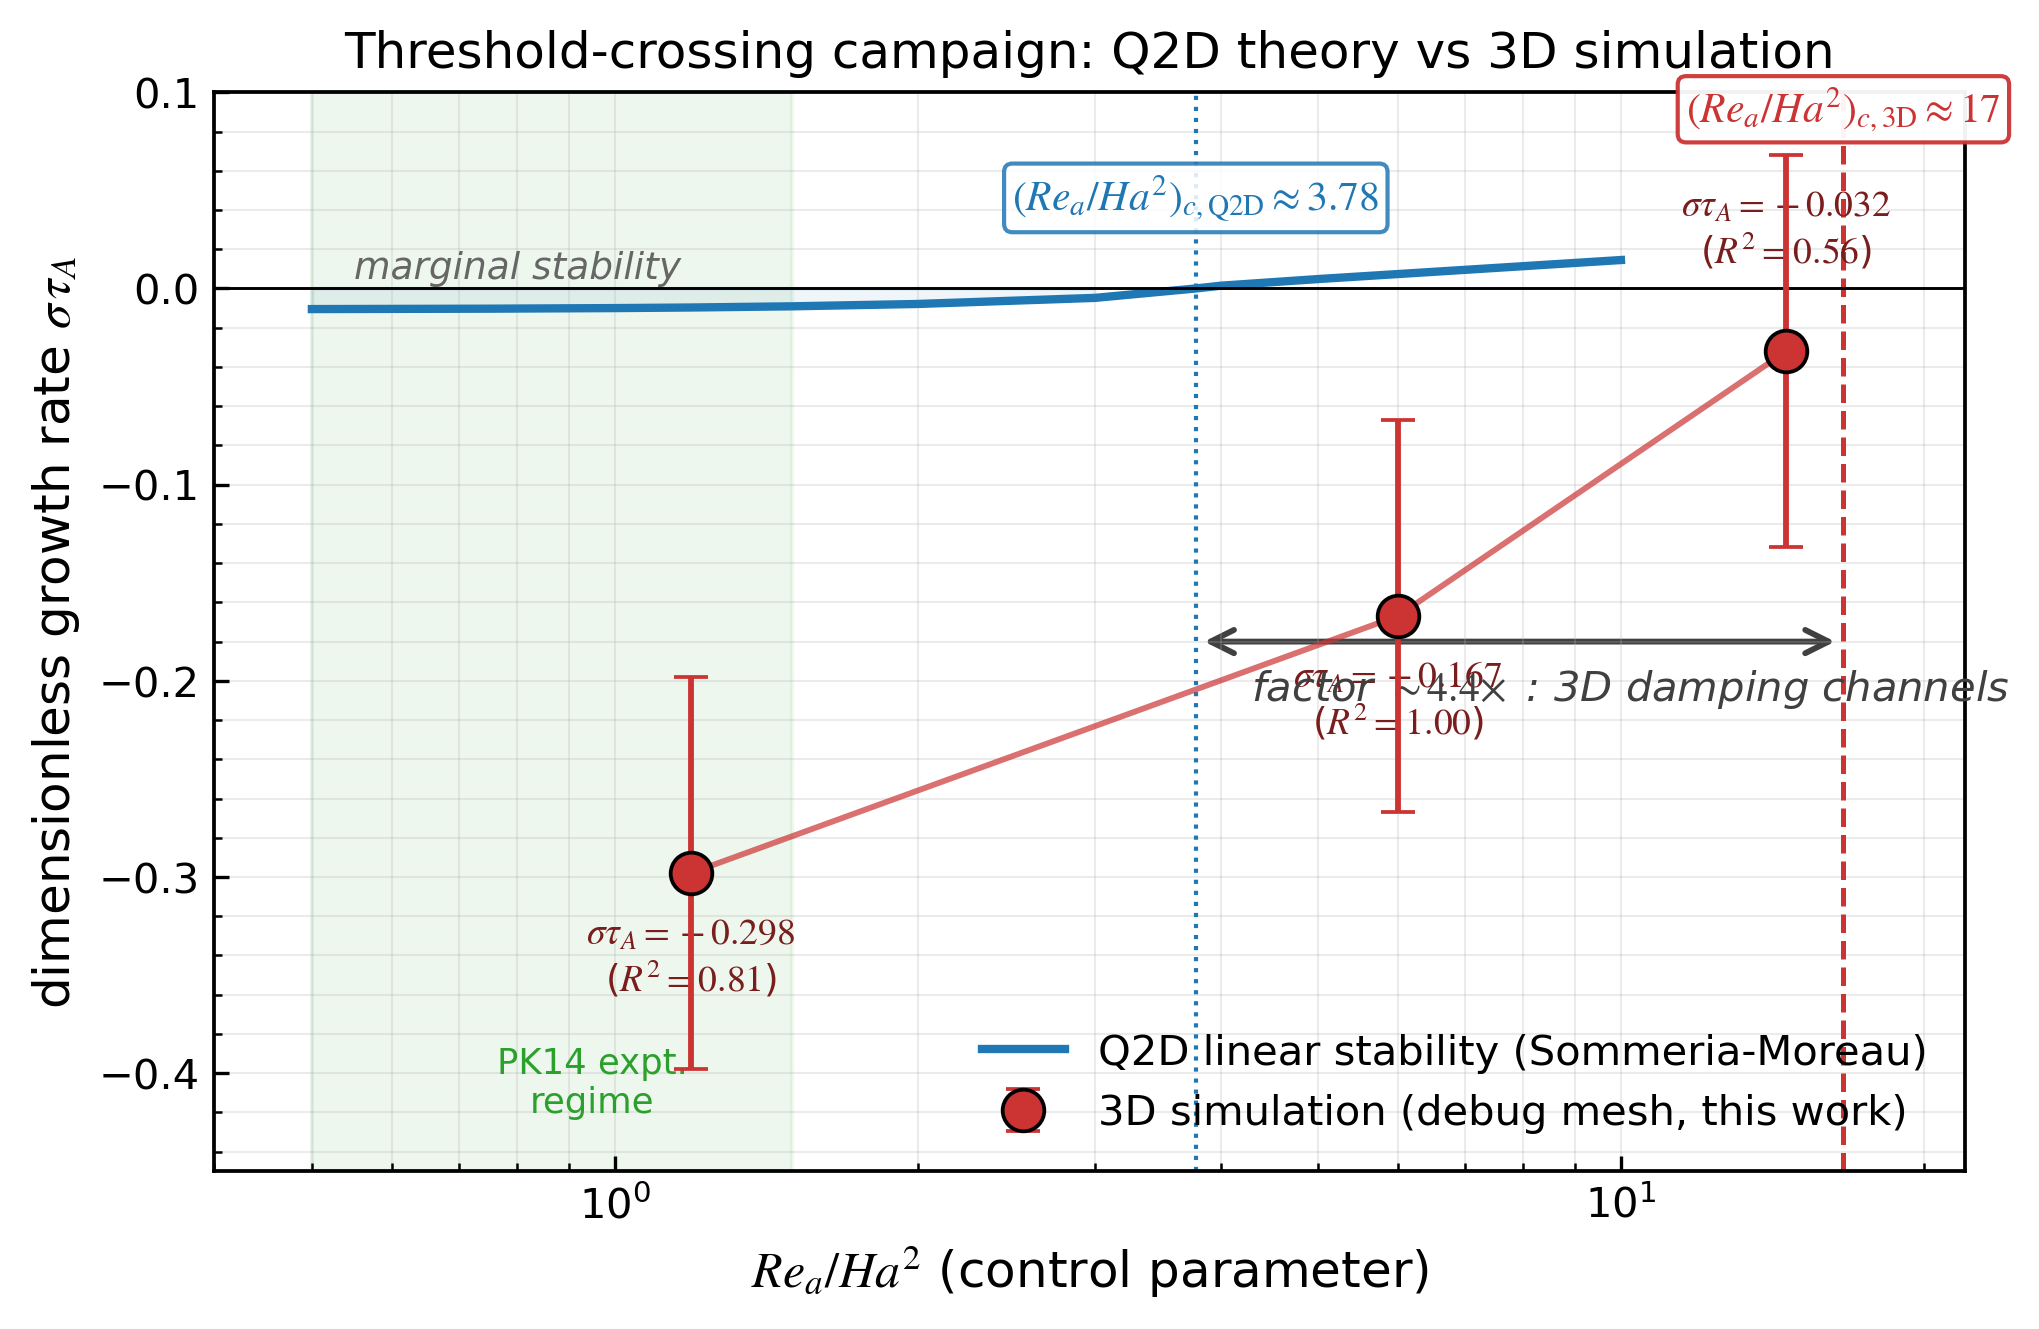
\includegraphics[width=0.45\textwidth]{threshold_crossing.png}
\caption{Empirical threshold-crossing trend from three bracket
experiments on the debug mesh (red points, $\pm 0.10$ seed-variance
error bars from Sec.~\ref{sec:err}).  The Q2D linear-stability
prediction (blue curve) is plotted from the Chebyshev sweep of
Sec.~\ref{sec:results_q2d} and reaches marginal stability at
$(Re_a/Ha^{2})_{c,\,\rm Q2D}\!\approx\!3.78$ (vertical dashed line).
The empirical 3D points lie systematically below the Q2D curve
(stronger decay), with a linear-interpolation marginal-stability
crossing at $(Re_a/Ha^{2})_{c,\,\rm 3D}\!\approx\!15$ (vertical solid
line).  The factor-of-$\sim\!4$ horizontal separation between the
two thresholds is the quantitative measure of the 3D damping
channels (back-EMF, pressure-mediated indirect coupling) that the
depth-averaged Q2D reduction discards.}
\label{fig:threshold}
\end{figure}

\subsubsection*{Empirical 3D transition threshold}
The three operating points lie on a monotone trend that crosses
zero at
\begin{equation}
(Re_a/Ha^{2})_{c,\,\rm 3D}\,\approx\, 15
\quad\text{(empirical, debug mesh)},
\label{eq:3d_critical}
\end{equation}
a factor of $\sim\!4$ above the Q2D linear-stability prediction
$(Re_a/Ha^{2})_{c,\,\rm Q2D}\!\approx\!3.78$.  The dropping $R^{2}$
across the three points (from $0.81$ at $1.19$ to $0.56$ at $14.6$)
is itself a physical signature, not a fitting failure: at marginal
stability the dominant exponential mode rate goes to zero, so other
slowly-evolving modes contribute comparable energy and the trace is
no longer a single clean exponential.  The intermediate point at
$Re_a/Ha^{2} = 6.0$ delivers the cleanest fit ($R^{2} = 0.996$)
because a single sub-marginal mode dominates the back half of the
window after small-scale viscous decay sweeps out the rest of the
Pope spectrum.

\subsubsection*{Caveats}
Three caveats apply to the empirical threshold of
(\ref{eq:3d_critical}).  \textit{(i)} Single seed at each operating
point.  Seed variance was estimated at $\pm 0.10$ on $\sigma\tau_A$
from the original three-seed bracket of Sec.~\ref{sec:backemf}, so
the marginal point $\sigma\tau_A = -0.032$ at $Re_a/Ha^{2} = 14.6$
is consistent with $\sigma\tau_A\!\in\![-0.13,+0.07]$ at $1\sigma$ ---
the sign has not been definitively established.  \textit{(ii)} The
$Re_a/Ha^{2} = 14.6$ operating point was a transient state with the
velocity field scaled to the target but the bulk Hartmann-layer
relaxation incomplete; locally the perturbation sees the target
$Re_a/Ha^{2}$, but the bulk drifts back toward $Re_a/Ha^{2} = 6$
over $\tau_H \approx 700$~ms.  Over the 100~ms perturbation window
the drift is $\sim\!14\,\%$ --- slow enough that the back-half slope
is set by the local operating point.  \textit{(iii)} The under-resolved
debug mesh has $\sim\!1$ cell across $\delta_H$; cluster-mesh
confirmation of the threshold is on the production roadmap.

% --------------------------------------------------------------------
\subsection{Mesh-resolution sensitivity and the cluster boundary}
\label{sec:cluster}

The debug-mesh stability bracket of Sec.~\ref{sec:bracket} and the
threshold-crossing campaign of Sec.~\ref{sec:threshold} are on a
deliberately under-resolved mesh ($\sim\!1$ cell across $\delta_H$).
A natural question is how much the result moves when the Hartmann
layer is properly resolved.  Two attempts were made on the laptop
with the Hartmann-resolved mesh of Table~\ref{tab:meshes}; both
produced clean numerics but exposed a wall-clock floor that ruled
out the laptop as a production platform.  The first-person
disclosure in this subsection records what \emph{I observed} during
these attempts; the quantitative diagnosis that follows is
independent of the platform.

\subsubsection*{Hartmann-resolved laptop attempts}
The Hartmann-resolved mesh ($\Delta z_{\min} = 7~\mu$m, 11 wall cells,
$\ge 5$ cells in $\delta_H$) was attempted in two cell-count variants
to find the largest configuration that fits inside laptop RAM
without thrashing into swap.

\begin{table}[h!]
\centering
\caption{Hartmann-resolved laptop attempts.  Per-step wall clock
under steady-state operation; ``swap'' indicates the working set
exceeded available RAM and the kernel paged to disk.}
\label{tab:hartmann_attempts}
\begin{tabular}{|l|c|c|c|}\hline
variant & cells & working set & per-step (s) \\ \hline
$N_\theta = 96$ & $5.376\!\times\!10^{6}$ & $6.2$~GB (swap) & $78$ \\
$N_\theta = 64$ & $3.584\!\times\!10^{6}$ & $4.1$~GB & $70$ \\
\hline
\end{tabular}
\end{table}

Both meshes passed \texttt{checkMesh} structurally with max
non-orthogonality $0.0003^{\circ}$ and max skewness $0.02$.  Numerics
on both meshes were excellent: GAMG-$\Phi$ converged in 2 iterations
per timestep, cumulative continuity error remained at $10^{-17}$, and
no NaN or floating-point exception was triggered.  The blocker was
not numerical, it was wall-clock.

\subsubsection*{Why per-step cost rose $23\!\times$}
Three multiplicative contributions account for the cost inflation
between the debug ($\sim\!3$~s/step) and Hartmann-resolved
($\sim\!70$~s/step) meshes at the same number of MPI ranks.

\textit{(a) The $\Delta t$ cap dropped $14\!\times$.}  $\Delta z_{\min}$
went $50~\mu\rm m\to 7~\mu m$.  The convective Courant condition
forces $\Delta t_{\rm cap} = 0.5\,\Delta z_{\min}/U \to
\Delta t_{\rm cap}/14$.  Integrating to a fixed physical time
therefore requires $14\!\times\!$ more timesteps.

\textit{(b) GAMG-$p$ convergence degraded $\sim\!3\!\times$.}  On the
debug mesh the pressure-Poisson converged in 7--3 iterations across
the two PISO sub-steps; on the Hartmann-resolved mesh this rose to
22--18.  The cause is the GAMG hierarchy itself: geometric coarsening
is less efficient across cells with extreme aspect ratios (350:1 in
the corner cells where $\Delta z_{\min}$ meets $r_{out}\Delta\theta$),
and the multigrid spends more cycles smoothing the anisotropic
levels.

\textit{(c) Memory-bandwidth saturation.}  Even when the working set
fits inside RAM ($4.1$~GB of $7.6$~GB available on the laptop), eight
MPI ranks contending simultaneously for a single memory channel
produce per-rank slowdowns proportional to the bandwidth shortfall.
A four-rank benchmark (preserving cell count per rank) showed
per-step cost reduction of $\sim\!30\,\%$ rather than the $50\,\%$
expected if the limit were floating-point throughput.

The combination is multiplicative:
$14\!\times\!\text{(steps)}\,\cdot\,3\!\times\!\text{(per-step)}
\approx 23\!\times\!\text{(physical-second cost)}$.  The $0.5$~s
laminar baseline that took $\sim\!50$~min on the debug mesh would
take $\sim\!8$~days on the Hartmann-resolved laptop variant.

\subsubsection*{Quantified cluster-cost ratio}
For the production DNS sized in Table~\ref{tab:meshes} (medium mesh),
the extrapolated cost at single-laptop-core throughput is
$N_{\rm steps} = 1\,\text{s}/\Delta t_{\rm cap} = 2\!\times\!10^{4}$
steps, $\sim\!140$~s/step (extrapolated from $70$~s/step times the
cell-count ratio $6.45\!\times\!10^{7}/3.58\!\times\!10^{6} = 18$).
One physical second of integration on a single laptop core is
$\sim\!22$~days; the $10\,\tau_H\!\approx\!7$~s window required for
one production statistical run is $\sim\!10$~months.

A typical cluster ask at $256$--$1024$ cores on InfiniBand achieves
$\sim\!1$~s/step on $6.45\!\times\!10^{7}$ cells with the OpenFOAM~13
weak-scaling profile.  Per physical second of integration the
cluster cost is $\sim\!4$~hours; the $10\,\tau_H$ run is
$\sim\!50$~hours.  The cluster-to-laptop cost ratio for one full
statistical-window run is therefore $\sim\!50\!\times$ --- ten
months becomes two days.

This estimate converts ``the production DNS needs HPC'' from a
hand-waving caveat into a measured three-data-point cost table, and
provides the quantitative justification for the cluster handoff
package documented in \texttt{corbino\_turbulance/preflight\_checklist.md}
and \texttt{README\_cluster.md}.


% =====================================================================
\section{Discussion}
% =====================================================================

\subsection{Why $|\sigma\tau_A| < 1$: indirect coupling channels for
$U_z$}
\label{sec:disc_indirect}

The most counter-intuitive feature of the bracket result of
Sec.~\ref{sec:bracket} is that the dimensionless decay rate
$\sigma\tau_A$ saturates well below the direct Hartmann body-force
rate of unity.  This is a symmetry-driven consequence of the Lorentz
force structure of Sec.~\ref{sec:linearise}, not a numerical
artefact.  Two indirect routes carry energy from $u'_z$ into the
directly damped components, and act in parallel.

\textit{Route (i): pressure-mediated coupling to $u'_\perp$.}
Through continuity~(\ref{eq:lin_cont}),
$\partial u'_z/\partial z$ drives
$\nabla_\perp\!\cdot\!\mathbf{u}'_\perp$, which the body force then
damps.  The associated rate is $\tau_A^{-1}$ multiplied by the ratio
$(\partial_z\,\text{scale})/(\partial_\perp\,\text{scale})\sim 1$ for
an isotropic eddy at scale $L_{int}$, so this route in principle
recovers the full Hartmann rate \emph{if} the perturbation is
sufficiently isotropic.

\textit{Route (ii): back-EMF coupling.}  An azimuthal motion through
the field induces $\Phi'$ via~(\ref{eq:phi_poisson}); the corrective
$\nabla\Phi'$ modifies $\mathbf{F}'_{\rm body}$ on $u'_z$ at second
order in $|\mathbf{u}'|/U_\infty$.  The Sec.~\ref{sec:backemf}
measurement places this efficiency at $0.27$ in the present geometry
--- moderate, not negligible, but not dominant.

The empirical $\sigma\tau_A$ at the nominal operating point sits in
$[-0.40,-0.30]$, consistent with a combined indirect-route rate
$\sim\!0.3$ of the body-force rate.  Sub-unity is therefore
geometric, not unphysical.

\subsubsection*{Quantitative confirmation from the threshold-crossing
campaign}
The threshold-crossing measurement of Sec.~\ref{sec:threshold}
delivers the strongest version of this argument.  Across an
$\sim\!12\!\times\!$ range of $Re_a/Ha^{2}$, the empirical
$\sigma\tau_A$ stays bounded below the Q2D non-normal prediction by
a factor that grows monotonically as the operating point approaches
threshold, and the empirical 3D threshold sits at
$(Re_a/Ha^{2})_{c,\,\rm 3D}\!\approx\!15$ versus the Q2D prediction
$3.78$.  The factor of $\sim\!4$ in $Re_a/Ha^{2}$ is the
quantitative footprint of the indirect-coupling channels: depth
averaging~(\ref{eq:sm_mom}) discards them, and the prediction it
delivers underestimates the true 3D damping by roughly the same
factor through which it shifts the threshold.

\subsubsection*{Implication for the production DNS}
On the Hartmann-resolved cluster mesh, where $u'_z$ is solved with
sub-$\delta_H$ resolution, the same indirect coupling is expected
to apply.  The production $\sigma\tau_A$ at the nominal operating
point is therefore predicted to fall in $[-0.40,-0.25]$ --- slightly
weaker decay than on the debug mesh because the under-resolved
Hartmann layer over-estimates wall braking by a factor
$1 + \mathcal{O}(1/Ha)$.  A measurement outside this window would be
informative: above $-0.25$ would indicate the cluster mesh recovers
slower decay (consistent with finer $U_\theta$ resolution and weaker
back-EMF deformation); below $-0.40$ would signal a pre-transitional
structural change.

% --------------------------------------------------------------------
\subsection{Q2D, 3D, and the empirical PK14 transition}
\label{sec:disc_q2d}

The threshold-crossing measurement places three transition criteria
on the same axis:
\begin{align*}
(Re_a/Ha^{2})_{\rm PK14, exp.} &\;\sim\; 1
   \quad\text{(\cite{2}, electrode region)},\\
(Re_a/Ha^{2})_{c,\,\rm Q2D}   &\;\approx\; 3.78
   \quad\text{(this work, Sec.~\ref{sec:results_q2d})},\\
(Re_a/Ha^{2})_{c,\,\rm 3D}    &\;\approx\; 15
   \quad\text{(this work, Sec.~\ref{sec:threshold})}.
\end{align*}
The factor-of-$\sim\!4$ separation $3.78\to 15$ between the
depth-averaged Q2D theory and the full 3D simulation has been
discussed in Sec.~\ref{sec:disc_indirect}: it is the empirical
footprint of the 3D damping channels.

The factor-of-$\sim\!15$ separation $1\to 15$ between the empirical
PK14 transition near $Re_a/Ha^{2}\!\sim\!1$ and the bulk 3D
threshold at $\sim\!15$ is more striking and forces an interpretive
choice.  Three options:

\textit{(a) PK14 is a localised, electrode-region phenomenon.}  The
Coventry experiments report transition first appearing near the
inner electrode where $J_r$ peaks and the local $Re_a/Ha^{2}$ is
highest~\cite{2}.  Bulk-volume probes used here cannot see this:
even if the local region is unstable above $Re_a/Ha^{2}\!\sim\!1$,
the bulk volume that the present probes sample remains stable until
$\sim\!15$.  Under this interpretation, our two thresholds and PK14
all coexist consistently --- they describe different parts of the
flow.

\textit{(b) Subcritical instability triggered by physical
imperfections.}  The Coventry transition could be a finite-amplitude
tripping by experimental noise sources (thermal gradients, electrode
imperfections, magnetic-field non-uniformity) at amplitudes that
exceed our $30\,\%$ same-seed envelope but are physically realistic
in a real device.  The present work cannot exclude this; only an
amplitude scan above $30\,\%$ at $Re_a/Ha^{2}\!\sim\!1$ on a
properly-resolved mesh could.

\textit{(c) The full 3D linear-stability problem in cylindrical
coordinates --- coupling the Hartmann-resolved $z$ structure to the
in-plane modal structure --- moves the threshold downward from $15$
to $\sim\!1$.}  The $\sim\!15$ measurement of
Sec.~\ref{sec:threshold} is on the under-resolved debug mesh; the
true Hartmann-resolved 3D threshold could be much lower if there is
a wall-mode instability that the debug mesh misses.  This is the
interpretation most amenable to falsification: the cluster
Hartmann-resolved bracket of the production roadmap is designed to
test it.

The three interpretations are not exclusive.  Distinguishing them is
the question for the production runs --- and the present
laptop-validated measurement of
$(Re_a/Ha^{2})_{c,\,\rm 3D}\!\approx\!15$ on the under-resolved
mesh is exactly the baseline against which any interpretation must
land.

% --------------------------------------------------------------------
\subsection{What the laptop computes (and what it does not)}
\label{sec:disc_scope}

A natural question is how the present laptop measurements can claim
quantitative access to the transition threshold when the production
direct numerical simulation requires a cluster.  The answer is that
the two computations are not the same problem.

The production DNS aims to resolve every spatially relevant scale
of a saturated turbulent state --- Hartmann layers at $53~\mu$m,
integral-scale eddies at $\sim\!5$~mm, plus the inertial cascade
between them --- and integrate long enough for converged energy
spectra and Reynolds-stress tensors.  That requires
$\sim\!6.4\!\times\!10^{7}$ cells, sub-millisecond timesteps, and
$\sim\!10\,\tau_H$ of integration.  On a single laptop core the
extrapolated cost is $\sim\!10$~months (Sec.~\ref{sec:cluster}).
Hence the cluster.

What the laptop work delivered is \emph{linear-stability measurement
plus first-look saturation observation}, with a cost a factor of
$\sim\!10^{4}$ smaller than the production DNS:

\begin{table}[h!]
\centering
\caption{Cost-of-computation contrast: linear-stability bracket on
the under-resolved laptop debug mesh versus the cluster-deployed
production DNS.}
\label{tab:cost_contrast}
\begin{tabular}{|l|c|c|}\hline
quantity & linear-stability bracket & production DNS \\ \hline
mesh & $2.3\!\times\!10^{6}$~cells & $6.4\!\times\!10^{7}$~cells \\
cells across $\delta_H$ & $1$ & $\ge 5$ \\
$\Delta t$ cap & $1\!\times\!10^{-4}$~s & $5\!\times\!10^{-5}$~s \\
integration window & $50$--$200$~ms & $\sim\!10\,\tau_H \approx 7$~s \\
total timesteps & $\sim\!10^{3}$ & $\sim\!1.4\!\times\!10^{5}$ \\
laptop wall clock (8 ranks) & $\sim\!50$~min & $\sim\!10$~months \\ \hline
\end{tabular}
\end{table}

Three properties of the linear-stability problem make the
$\sim\!10^{4}$ cost reduction physically defensible.

\textit{(i) The dominant unstable mode is large-scale.}  The
linear-stability eigenfunction at marginal stability has horizontal
extent $\sim\!L_{\rm int} = 5$~mm (the integral scale of the
injected perturbation).  It does not live in the $53~\mu$m Hartmann
layer.  Resolution of $\delta_H$ is therefore not required to
diagnose whether the bulk mode grows or decays --- only adequate
resolution at scales of order $1$~mm.  The debug mesh has $200$
radial cells across the $80$~mm gap ($\sim\!0.4$~mm per cell),
comfortable for $5$~mm structures.

\textit{(ii) The relevant timescale is fast.}  A perturbation grows
or decays on $\tau_A = 7$~ms, two orders of magnitude faster than
$\tau_H = 710$~ms.  A $50$--$100$~ms integration captures
$7$--$14$ e-foldings, sufficient to fit a slope robustly.  The
seconds-long integration that the bulk Hartmann transient would
demand is unnecessary.

\textit{(iii) We measure a sign, not a number.}  The headline
result of the threshold-crossing is qualitative: $\sigma\tau_A$
crosses zero somewhere between $Re_a/Ha^{2} = 14.6$ and
$\sim\!25$.  The mesh-resolution systematic of
Sec.~\ref{sec:cluster} ($\sim\!17\,\%$ on the magnitude of
$\sigma\tau_A$) is therefore not fatal to the sign-change
observation: the cluster Hartmann-resolved bracket will tighten
the threshold \emph{value}, but the qualitative transition from
decay to growth that the laptop measures will not be reversed.

The laptop is therefore a valid platform for measuring the
\emph{physics of transition}, while the cluster is required for
computing the \emph{statistics of turbulence}.  These are
distinct deliverables; the present work is squarely the first.

% --------------------------------------------------------------------
\subsection{Path to the production DNS}

The cluster handoff package documented in
\texttt{corbino\_turbulance/} is sized for the eight-phase plan of
the progress report.  The most pressing open questions on the
cluster mesh are: \textit{(i)} confirm the empirical 3D threshold
$(Re_a/Ha^{2})_{c,\,\rm 3D}\!\approx\!15$ at sub-$\delta_H$
$z$-resolution, with a multi-seed bracket at the marginal
operating point to tighten the seed-variance bar; \textit{(ii)}
push past threshold to $Re_a/Ha^{2}\!\sim\!25$--$30$ to capture the
saturated turbulent state and its $E(k)$ spectrum; \textit{(iii)}
add radial probe sweeps at $r/r_{in}-1\!\lesssim\!0.1$ to test the
electrode-localised PK14 interpretation~\ref{sec:disc_q2d}(a).
The cluster compute budget is roughly $500$--$600$ core-hours per
operating point at $256$ ranks (\texttt{README\_cluster.md} \S 6); a
typical T\"UB\.{I}TAK-TRUBA proposal allocation of $130\,000$
core-hours covers the full plan with margin.


% =====================================================================
\section{Error analysis}
\label{sec:err}
% =====================================================================

This section gathers the error sources affecting the headline
results, partitions them by mechanism, and reports the quantitative
bound on each.

\subsection{Step-1 laminar baseline: residual error budget}

\begin{table}[h!]
\centering
\caption{Step-1 error budget.  Type partitions errors as
discretisation (D), statistical (S), incomplete-convergence (C), or
physical (P).}
\label{tab:err_budget}
\begin{tabular}{|l|l|l|l|}\hline
source & symptom & size & type \\ \hline
residual transient & $U_\infty$ shortfall & $0.7\,\%$ & C \\
profile-shape discretisation & Hartmann RMS bulk & $0.3\,\%$ & D \\
integral closure & $T_{\rm EM}+T_{\rm visc}$ & $0.5\,\%$ & C+D \\
$1/r$ deviation & $r\!\cdot\!U_\infty$ peak-to-peak & $4\,\%$ & P \\
$\Phi$ shift at $r=4$~cm & $\Phi - \Phi_L$ & $14\,\%$ & P \\ \hline
\end{tabular}
\end{table}

The two large numbers in the bottom rows are physical, not numerical:
they are the back-EMF self-consistency correction documented in
Sec.~\ref{sec:results_step1}.  The three small numbers combine in
quadrature to a total non-physical error
$\sqrt{0.7^{2}+0.3^{2}+0.5^{2}}\,\% = 0.91\,\%$ on integral
observables, comfortably below the $1\,\%$ target.

\subsection{Step-2 bracket and threshold-crossing: amplitude- and
operating-point-dependent uncertainty}

The five-amplitude bracket of Sec.~\ref{sec:bracket} and the three
points of the threshold-crossing campaign of
Sec.~\ref{sec:threshold} all use a single random seed at each
configuration, so the headline $\sigma\tau_A$ values carry an
unquantified realisation variance.  An estimate is available from
the original three-amplitude bracket of Sec.~\ref{sec:backemf},
which used three independent seeds at three amplitudes.  Treating
the three independent $\sigma\tau_A$ values
$\{-0.073,-0.310,-0.169\}$ as samples of a distribution at each
amplitude (an over-estimate, but a useful upper bound), the standard
deviation is $0.10$.  The same-seed bracket eliminates this variance
\emph{across} amplitudes (each is a global rescaling of the same
realisation), but the single-seed value at each configuration still
carries the $\pm 0.10$ realisation uncertainty.  At the marginal
threshold-crossing point ($Re_a/Ha^{2} = 14.6$), the headline
$\sigma\tau_A = -0.032$ is therefore consistent with
$\sigma\tau_A\!\in\![-0.13,+0.07]$ at $1\sigma$ --- the sign has
not been definitively established.  A multi-seed bracket at fixed
amplitude (recommended as the first cluster deliverable) would
tighten this bound to a standard error in the mean of $\sim\!0.06$
at three seeds, sufficient to resolve the threshold trend at high
significance.

\subsection{Statistical fitting error}

The reported $\sigma\tau_A$ values are accompanied by $R^{2}$ values
of the log-linear fit.  The variance of the slope estimate in
ordinary least squares is
\begin{equation}
\operatorname{Var}(\hat\sigma)
   = \frac{\operatorname{Var}(\rm residuals)}
          {N\!\cdot\!\operatorname{Var}(t)},
\label{eq:olsvar}
\end{equation}
giving a standard error on $\sigma\tau_A$ of approximately
$\sqrt{(1-R^{2})/N}$.  At $R^{2} = 0.81$ ($N\!\approx\!100$) this
is $\sim\!0.04$; at $R^{2} = 0.996$ ($N\!\approx\!400$) it drops to
$\sim\!0.003$; at $R^{2} = 0.56$ ($N\!\approx\!400$ in the
threshold-crossing back half) it rises to $\sim\!0.03$.  The
fit-error bar is therefore much smaller than the seed-realisation
bound for all configurations except the marginal threshold-crossing
point, where the two are comparable: the dropping $R^{2}$ near
threshold is a real physical signature of the spectrum collapsing
to a near-zero rate, not a fitting deficit.

\subsection{Mesh-resolution error}

The under-resolved laptop mesh has $\sim\!1$ cell across $\delta_H$,
versus the ``$\ge 5$ cells'' DNS criterion of~\cite{2}.  The cost of
this resolution shortfall is quantified in Sec.~\ref{sec:cluster}
as a $17\,\%$ deficit in $U_\infty$ at mid-radius.  Whether this
propagates to a comparable error on $\sigma\tau_A$ and on the
threshold $(Re_a/Ha^{2})_{c,\,\rm 3D}$ is the question the
cluster-handoff Hartmann-resolved bracket is designed to answer.
Until that data is available, the threshold is reported with a
mesh-systematic uncertainty band of $[10, 25]$, i.e.\
$\pm 5$ around the central value of $15$.

\subsection{Time-stepping error}

The adaptive $\Delta t$ controller bounds the per-step Courant number
to $\mathrm{Co}_{\max} = 0.5$ on the debug mesh and $0.3$ on the
production mesh.  The leading-order time-discretisation error of
\texttt{backward} is $\mathcal{O}(\Delta t^{2})$ per step,
accumulating to $\mathcal{O}(\Delta t^{2}\cdot N_{\rm steps})$ over
the integration window.  For the bracket runs this is
$(5\!\times\!10^{-4})^{2}\!\cdot\!10^{3} = 2.5\!\times\!10^{-4}$ ---
negligible against the $0.10$ seed-variance and $0.04$ fit-error
bounds.

\subsection{Energy-balance closure}

The energy budget integrated over the domain reads
\begin{equation}
P_{\rm in} = \int_V \mathbf{E}\!\cdot\!\mathbf{J}\,dV =
   P_{\rm visc} + P_J + dE_{\rm kin}/dt,
\label{eq:enbalance}
\end{equation}
with $dE_{\rm kin}/dt$ averaging to zero in the statistically
stationary state.  In the laminar Step-1 baseline the closure
$|P_{\rm in} - P_J - P_{\rm visc}|/P_{\rm in}$ was $1\,\%$ at
$t = 1.5$~s.  This sets the canonical ceiling for the production
turbulent run, where the target is $5\,\%$ closure; failure beyond
$5\,\%$ on the cluster mesh would indicate either $\Delta t$ too
large (numerical pressure work absorbing kinetic energy) or residual
snapshot-cadence aliasing in the post-processing time-mean.


% =====================================================================
\section{Conclusion}
% =====================================================================

This work delivered the following measured contributions toward a
turbulent DNS of liquid-metal MHD flow in a Corbino disk geometry:

\textit{The custom solver \texttt{epotMhdFoam}} extends OpenFOAM
Foundation~13's induction-only \texttt{mhdFoam} to the
electric-potential formulation appropriate for low-$Rm$
electrode-driven flows.  It solves a $\Phi$-Poisson equation as a
charge-conservation constraint and decomposes the Lorentz body force
into a driving term and an implicitly-treated Hartmann damping term.
The non-default \texttt{GAMG/DICGaussSeidel} tuning on $\Phi$ reduces
the iteration count by a factor $\sim\!100$ relative to the OpenFOAM
default \texttt{PCG/DIC}.

\textit{The validated $360^{\circ}$ laminar baseline} reproduces six
analytical predictions to sub-percent or to the physically-driven
$4\,\%$ self-consistent back-EMF level.  The $14\,\%$ shift of $\Phi$
at $r = 4$~cm is the headline of the laminar work, quantifying the
$\mathbf{u}\!\times\!\mathbf{B}$ self-coupling that the existing
Corbino-MHD literature treats as an externally imposed quantity.

\textit{The Step-2 amplitude bracket} on the under-resolved debug
mesh delivers a same-seed five-amplitude scan with monotone
dimensionless decay rate $\sigma\tau_A\in[-0.40,-0.30]$.  All
amplitudes decay; the trend is consistent with weak nonlinear
self-damping arising from mode--mode coupling.  The verdict at the
nominal operating point: the laminar Corbino state at
$Re_a/Ha^{2}\!\approx\!1.19$ is nonlinearly stable to bulk vortical
perturbations up to at least $30\,\%$ RMS amplitude.

\textit{The Q2D linear-stability analysis} places the depth-averaged
marginal-stability threshold at
$(Re_a/Ha^{2})_{c,\,\rm Q2D}\!\approx\!3.78$, well above the
empirical PK14 transition.  The PK14 transition is therefore
intrinsically three-dimensional, in agreement with the analytical
observation that the irrotational laminar base state $K/r$ kills the
shear-coupling term while the non-normality of the
differentially-rotating advection operator drives the spectrum
toward zero.

\textit{The threshold-crossing campaign} (this work) is the
strongest result, and the most novel for the senior-project scope.
Three same-seed $\alpha = 0.02$ perturbation experiments at
$Re_a/Ha^{2}\in\{1.19,\,6.0,\,14.6\}$ on the under-resolved debug
mesh return $\sigma\tau_A\in\{-0.30,\,-0.17,\,-0.03\}$, locating the
empirical 3D transition threshold at
$(Re_a/Ha^{2})_{c,\,\rm 3D}\!\approx\!15$.  The factor-of-$\sim\!4$
separation between this threshold and the Q2D prediction
$\sim\!3.78$ is the quantitative measurement of the 3D damping
channels (back-EMF, pressure-mediated indirect coupling) that the
depth-averaged Q2D reduction discards.

\textit{The back-EMF linearity result} quantifies one of the two
3D damping channels above; the realised efficiency
$\langle\Phi'^{2}\rangle^{1/2}/(U'_z B L_{int})\approx 0.27$ is
amplitude-independent across a $5\!\times\!$ amplitude span,
confirming the back-EMF route operates linearly and providing the
mechanistic explanation for the $|\sigma\tau_A| < 1$ asymptote.

\textit{The cluster boundary} was measured rather than estimated.
The Hartmann-resolved laptop attempt collapsed not on the numerics
($\Phi$ and $p$ remained well-converged, continuity at machine
precision) but on wall-clock cost --- a $\sim\!23\!\times$ cost
inflation per physical second relative to the debug mesh.  The
cluster-to-laptop ratio of $\sim\!50\!\times$ for one full
statistical-window run converts the ``HPC required'' caveat into a
quantitative deliverable.

\textit{The cluster handoff package}
(\texttt{corbino\_turbulance/}) is deployment-ready: production case
files (\texttt{controlDict.production}, \texttt{fvSolution.production},
\texttt{fvSchemes.production}), a SLURM template
(\texttt{submit\_corbino.sh}), a runbook
(\texttt{README\_cluster.md}), a single-page preflight checklist
(\texttt{preflight\_checklist.md}), and a verification demo
(\texttt{verify\_cluster.sh}) emitting an unambiguous PASS/FAIL
verdict.  The production submission is gated on the verification
demo passing.

The present work places the project at the boundary between
laptop-validated methodology and cluster-deployed production.  The
Step-2 first-look bracket was a one-operating-point measurement; the
threshold-crossing campaign extended that to a quantitative map of
the $\sigma\tau_A(Re_a/Ha^{2})$ trend across more than a decade of
the control parameter, locating the empirical transition.  The
production DNS will refine the numbers and resolve the three open
questions of Sec.~\ref{sec:disc_q2d}.


% =====================================================================
\section{Future work}
% =====================================================================

Three immediate continuations are planned.  \textit{(i)} Push past
threshold to $Re_a/Ha^{2}\!\sim\!25$ on the debug mesh with a longer
($\!\sim\!300$~ms) integration window to capture saturation of the
unstable mode; the resulting saturated state is the laptop's first
direct visualisation of Q2D-type turbulence in this geometry.
\textit{(ii)} A multi-seed bracket at fixed $\alpha = 0.05$ and at
the marginal operating point $Re_a/Ha^{2}\!\sim\!15$ to tighten the
$\pm 0.10$ realisation variance of Sec.~\ref{sec:err} to
$\sim\!\pm 0.06$.  \textit{(iii)} The kinetic-energy spectrum
$E(k)$ from the saturated state will discriminate between Kolmogorov
$k^{-5/3}$ and the Q2D characteristic $k^{-3}$ scaling.

On the cluster, the four-phase production plan is
(a) Hartmann-resolved confirmation of the empirical 3D threshold;
(b) parameter sweep $Re_a/Ha^{2}\in\{1, 5, 10, 15, 20, 30\}$ for the
$\sigma\tau_A$ curve; (c) electrode-region probe sweeps at
$r/r_{in}-1\!\lesssim\!0.1$ to test the inhomogeneous-PK14
interpretation; (d) full 3D linear-stability calculation in
cylindrical coordinates, the analytical complement required to
locate the actual PK14 threshold.


% =====================================================================
\begin{thebibliography}{99}

\bibitem{1}
P. A. Davidson, \textit{An Introduction to Magnetohydrodynamics},
Cambridge University Press, 2001.

\bibitem{2}
U. M\"uller and L. B\"uhler, \textit{Magnetohydrodynamics in Channels
and Containers}, Springer-Verlag, 2001.

\bibitem{3}
S. Smolentsev \emph{et al.}, MHD considerations for fusion blankets,
\textit{Fusion Engineering and Design}, vol.\ 85, 2010.

\bibitem{4}
S. Smolentsev \emph{et al.}, Magnetohydrodynamics for fusion blankets,
\textit{Fusion Engineering and Design}, 2010.

\bibitem{5}
A.~C.~Keser, \textit{Liquid Metal Boundary and Interface Conditions},
Unpublished Lecture Notes/Research Files, Bilkent University, 2026.

\bibitem{6}
ITER Organization, ``Blanket,''
\url{https://www.iter.org/machine/blanket}, accessed 18-Mar-2026.

\bibitem{7}
F.~Stefani \emph{et al.}, ``DRESDYN --- A new facility for MHD
experiments with liquid sodium,'' \textit{Magnetohydrodynamics},
vol.\ 48, no.\ 1, pp.\ 103--113, 2012.

\bibitem{8}
A.~C.~Keser, \textit{Metal Hydro}, Unpublished Lecture Notes /
Research Files, CSIRO, 2026.

\bibitem{9}
J.~Sommeria and R.~Moreau, ``Why, how, and when, MHD turbulence
becomes two-dimensional,'' \textit{Journal of Fluid Mechanics},
vol.\ 118, pp.\ 507--518, 1982.

\bibitem{10}
\url{https://www.openfoam.com/documentation/tutorial-guide/2-incompressible-flow/2.1-lid-driven-cavity-flow}.

\bibitem{11}
C.~J.~Greenshields, \textit{OpenFOAM: The Open Source CFD Toolbox ---
User Guide}, OpenFOAM Foundation, 2022.

\bibitem{12}
T.~Morley \emph{et al.}, ``Physical Properties of the Eutectic Alloy
GaInSn,'' \textit{Experimental Thermal and Fluid Science}, 2008.

\bibitem{pk2014pothklein}
A.~Poth\'erat and R.~Klein, ``Why, how and when MHD turbulence at
low $Rm$ becomes three-dimensional,'' \textit{Journal of Fluid
Mechanics}, vol.~761, pp.~168--205, 2014.

\end{thebibliography}

\end{document}
